%\documentclass[9pt,shortpaper,twoside,web]{ieeecolor}
%\documentclass[journal,twoside,web]{ieeecolor}
%\documentclass[runningheads]{llncs}
%\usepackage{cite}
%\usepackage{amsmath,amssymb,amsfonts}
%\usepackage{algorithmic}
%\usepackage{graphicx}
%\usepackage{textcomp}
%\usepackage{multicol}
%\usepackage{multirow}
%\usepackage{subcaption}
%\usepackage{amsfonts}
%\usepackage{listings}
%\usepackage{authblk}
%\usepackage[hidelinks]{hyperref}
%\usepackage[table,xcdraw]{xcolor}
%\usepackage{float}

\documentclass[11pt,letterpaper,english]{article}
 \usepackage[table,xcdraw]{xcolor}
\usepackage{enumitem}
\usepackage[font=bf]{caption}
\usepackage{sectsty}
\usepackage{pslatex}
\usepackage[margin=1in]{geometry}
\usepackage{url}
\usepackage{listings}
\usepackage{wrapfig}
\usepackage{booktabs}
%\usepackage{color}
%\usepackage{xcolor}
\usepackage{graphicx}
%\usepackage{subfigure}
\usepackage{epsfig}
\usepackage{multirow}
\usepackage{verbatim}
\usepackage{epstopdf}
\usepackage{fancyhdr}
\usepackage{setspace}
\usepackage{array}
\usepackage{amsmath}
%\usepackage{algorithmic}
%\usepackage{algorithm}
\usepackage{multicol}
%\usepackage{bibunits}
%\usepackage{setspace}
%\usepackage{epstopdf}
%\usepackage{amsmath}
%\usepackage{pdfsync}
%\usepackage{fullpage}
%\usepackage{hyperref}
%\usepackage{bigstrut}
%\usepackage{mathrsfs}
\usepackage{amssymb}
%\usepackage[compact]{titlesec}
%\usepackage{pslatex}
\usepackage{tikz}
\usepackage{graphicx}
\usepackage{caption}
\usepackage{wrapfig,lipsum,booktabs}
\usepackage{subcaption}

\usepackage[utf8]{inputenc}
\usepackage{enumitem}



%\usepackage{changes} % to highlight the changes
\newcommand{\change}[1]{\textcolor{red}{#1}}


\begin{document}
\title{Lorem ipsum dolor sit amet, consectetur adipiscing elit, sed do eiusmod tempor incididunt ut labore et}
\pagestyle{empty}

\author{Ahmedur Rahman Shovon~$^\star$, Sidharth Kumar \thanks{Ahmedur Rahman Shovon (email: ashovon@uab.edu) and Sidharth Kumar (email: sid14@uab.edu) are at the computer science department of University of Alabama at Birmingham, Birmingham, AL 35294 USA.}
, Gopikrishna Deshpande \thanks{Gopikrishna Deshpande is at AU MRI Research Center, Department of Electrical and Computer Engineering, Auburn University, AL, USA. He is also affiliated with the following: (a) Department of Psychological Sciences, Auburn University, Auburn, USA (b) Alabama Advanced Imaging Consortium, Birmingham, USA, (c) Center for Neuroscience, Auburn University, USA, (d) School of Psychology, Capital Normal University, Beijing, China, (e) Key Laboratory for Learning and Cognition, Capital Normal University, Beijing, China, (f) Department of Psychiatry, National Institute of Mental Health and Neurosciences, Bangalore, India and (g) Centre for Brain Research, Indian Institute of Science, Bangalore, India. (e-mail: gzd0005@auburn.edu)}
}
%\institute{}


%\author{Sidharth Kumar\inst{1} \and
%Ahmedur Rahman Shovon\inst{1} \and
%Gopikrishna Deshpande\inst{2}}

%\institute{University of Alabama at Birmingham, Birmingham AL 35233, USA \and
%Auburn University, Auburn, AL 36849, USA\\
%\email{lncs@springer.com}}



%\author{Sidharth Kumar, \IEEEmembership{Member, IEEE}, and Gopikrishna Deshpande,\IEEEmembership{Member, IEEE}

%\thanks{This paragraph of the first footnote will contain the date on which
%you submitted your paper for review. It will also contain support %information,
%including sponsor and financial support acknowledgment. For example, 
%``This work was supported in part by the U.S. Department of Commerce under %Grant BS123456.'' }
%\thanks{Sidharth Kumar is at computer science department of University of Alabama at Birmingham, Birmingham, AL 35294 USA (e-mail:sid14@uab.edu). }
%\thanks{Gopikrishna Deshpande is at AU MRI Research Center, Department of Electrical and Computer Engineering, Auburn University, AL, USA. He is also affiliated with the following: (a) Department of Psychological Sciences, Auburn University, Auburn, AL, USA (b) Alabama Advanced Imaging Consortium, Birmingham, AL, USA, (c) Center for Neuroscience, Auburn University, AL, USA, (d) School of Psychology, Capital Normal University, Beijing, China, (e) Key Laboratory for Learning and Cognition, Capital Normal University, Beijing, China, (f) Department of Psychiatry, National Institute of Mental Health and Neurosciences, Bangalore, India and (g) Centre for Brain Research, Indian Institute of Science, Bangalore, India. (e-mail: gzd0005@auburn.edu)}}
\date{}

\maketitle



\vspace{-0.4cm}
\begin{abstract}
Based on functional connectivity networks (FCN) discovered from resting-state functional magnetic resonance imaging (rs-fMRI), the study of brain function is gaining popularity. FCNs are susceptible to factors affecting data acquisition parameters, such as the temporal sampling period. The difference in temporal sampling rates of MRI machines negates the benefits of larger sample sizes in pooled data by introducing non-neural variability in the collected data. Preserving the topology of the FCN for different sampling periods can mitigate this issue. We use Persistent Homology (PH) to preserve the topology of the FCNs from different temporal sampling periods. Persistent homology can extract topological features which outperform graph analytics by preserving the network topology for continuous time series data. The persistent diagrams represent the topological features and are compared using the Wasserstein distance metric. We presented a novel Topological Data Analysis (TDA) framework that is applied on $371,616$ adjacency matrices extracted from three temporal sampling periods ($2500ms$, $1400ms$, $645ms$) of rs-fMRI datasets collected from 316 subjects proving the robustness of persistent homology to a specific data acquisition parameter (temporal sampling period). Using statistical analysis, we evaluated the resiliency of our TDA framework on different temporal sampling periods of rs-fMRI datasets.


% There is increasing interest in investigating brain function based on functional connectivity networks (FCN) obtained from resting-state functional magnetic resonance imaging (fMRI). FCNs, typically obtained using measures of time series association such as Pearson’s correlation, are sensitive to data acquisition parameters such as sampling period. This introduces non-neural variability in data pooled from different acquisition protocols and MRI scanners, negating the advantages of larger sample sizes in pooled data. To address this, we hypothesize that the topology or shape of brain networks must be preserved irrespective of how densely it is sampled, and metrics which capture this topology may be statistically similar across sampling periods, thereby alleviating this source of non-neural variability. Accordingly, we present an end-to-end pipeline that uses persistent homology, a branch of topological data analysis, to demonstrate \emph{similarity} across FCNs acquired at different temporal sampling periods. Persistent homology (PH) as a technique extracts topological features by capturing the network organization across all continuous threshold values, as opposed to graph theoretic methods, which fix a discrete network topology by thresholding the connectivity matrix. The extracted topological features are encoded in the form of persistent diagrams that can be compared against one another using the earth-moving metric, also popularly known as the Wasserstein distance. We extract topological features from three data cohorts, each acquired at different temporal sampling periods and demonstrate that these features are statistically the same, hence, empirically showing that PH is invariant to data acquisition parameters such as sampling period. 
\end{abstract}

%\begin{keywords}
%Topological data analysis, TDA, fMRI, Persistent homology
%\end{keywords}

\section{\textcolor{red}{Introduction}}
\label{sec:introduction}
\change{
Studying the functional and anatomical connectivity of the human brain has given us a deeper understanding of the characteristics of the brain, from microscale connectivity between single neurons to macroscale connectivity between regions of interest in whole brain images. One of the routinely employed approaches for characterizing macroscale connectivity utilizes measures of statistical association (such as Pearson’s correlation) obtained from resting-state functional magnetic resonance imaging (rs-fMRI) times series corresponding to specific ROIs in the human brain. The connectivity matrix thus obtained is an algebraic representation of the weighted brain network, which shows the relationship between all pairs of nodes. } 

\change{Functional connectivity obtained from rs-fMRI has been shown to be extremely sensitive to mental health disorders~\cite{fornito2010can} as well as predictive of behavior in healthy individuals~\cite{miller2016multimodal}. This has kindled interest in using functional connectivity networks (FCNs) as potential biomarkers of mental disorders. The sensitivity and specificity of these biomarkers and their generalizability to the general population seem to increase with sample size. However, acquiring data from larger samples at any given site can be economically and logistically prohibitive. Therefore, there has been a recent impetus toward post-hoc aggregation of data acquired at different sites to form larger datasets. Examples include the Autism Brain Imaging Data Exchange (ABIDE~\cite{di2014autism}) and ADHD-200~\cite{bellec2017neuro}. In such large publicly available datasets, it has been found that biomarkers do not generalize well to data acquired at different sites. This has been attributed to the fact that MRI scanners and data acquisition protocols are different across sites, and this induces an element of non-neural variability in the data that tends to make it difficult for us to discover consistent inter-group FCN differences that are at least partly neural in origin. 
}

Functional brain imaging studies are increasingly utilizing topological data analysis (TDA), a mathematical approach grounded in algebraic topology~\cite{das2022topological}. 



Traditionally, graph-theoretic tools, which can be construed as special cases of the more generic concepts of TDA, have been extensively used to study and quantify FCNs. More recently, advanced tools from TDA such as persistent homology (PH)~\cite{rubinov2010complex} have been used to study complex networks. Persistent homology investigates connections between different parts of networks using algorithms designed to encode and measure the significance of relationships across multiple scales (thresholds). In the context of networks, topological features refer to the $0-$, $1-$, $2-$ dimensional homology groups of a metric space that describe its \emph{connected components}, \emph{tunnels}, and \emph{voids} respectively. Most graph-theoretic techniques can quantify these features of a weighted brain network only at a fixed threshold. PH provides a principled approach to quantifying these features for all thresholds; more precisely, it can track when features (such as connected components, loops, and voids) are created and destroyed with varying scales (threshold). The technique quantifies the individual topological events (birth and death of features) in the graph according to their significance (or persistence). This persistence is represented in the form of barcodes, which encode the threshold at which features appear and disappear. The barcodes encode these sets of features can be seen as a fingerprint for a graph. What makes this fingerprint useful is the presence of metrics such as Wasserstein distance (WD)~\cite{vallender1974calculation, edelsbrunner2013persistent} that can be used to quantify the statistical difference between two barcodes robustly. The WD is robust to small perturbations in the data and hence can be used to compare and establish similarities between persistent diagrams. We use this ability in our pipeline to establish similarities between barcodes obtained from brain networks derived from data acquired with different acquisition parameters (such as sampling period).


The input to our TDA-based pipeline is subject-specific FCNs from three data cohorts, corresponding to data acquired from the same individuals at three different sampling periods (TR):  645ms, 1400ms and 2500ms. The cohort consists of rs-fMRI data from 316 subjects (totaling $3 \times 316$ scans). In our pipeline, %first, each FCN instance is embedded into a metric space that sets it up for TDA. Following this, 
the topological features of each network instance are extracted using persistent homology and encoded with a barcode. The barcodes are compared against each other by using the Wasserstein distance (WD). In particular, we perform two sets of experiments to demonstrate that the FCNs indeed capture the same structure irrespective of the temporal sampling periods: (a) making a direct pairwise comparison of the same subjects across different temporal sampling periods and (b) performing pairwise comparison within a cohort (same temporal sampling period) to extract the overall pattern of subjects and then comparing that pattern across the sampling periods. The statistical analysis is made possible because the barcodes (our metric) can be compared against one another using the WD~\cite{vallender1974calculation, edelsbrunner2013persistent}. 
In our first set of experiments, we perform pairwise WD computation of the same subjects but between different sampling periods (across the data cohorts), and this yields $3$ groups of measurements: WD between ($645$ms and $1400$ms), ($1400$ms and $2500$ms) and ($2500$ms and $645$ms). We then demonstrate similarity among these distributions by performing ANOVA and t-tests, further establishing the invariance that FCNs capture the same information, irrespective of the data acquisition parameters.
In our second set of experiments, we calculate pairwise WD between persistence diagrams of all $316$ subjects. This yields three sets of adjacency matrices (one for every sampling rate); we perform multidimensional scaling (MDS)~\cite{carroll1998multidimensional, cox2008multidimensional} on this high dimensional data, reduce it to a 2D space and then apply clustering techniques to segregate the subjects into clusters. Finally, we compare the number of clusters across the three cohorts. In particular, our paper makes the following three contributions to the literature:
\begin{enumerate}
\item Demonstrate that the barcode obtained from the PH of resting state fMRI data is a compact representation of topological information of an FCN.
\item Present an end-to-end pipeline that uses PH-based techniques to demonstrate that FCN networks are invariant to data acquisition parameters such as temporal sampling periods (TR), potentially removing a source of noise in multi-site case-control studies, thereby improving the effect sizes in group comparisons. 
\item Present an open-source and reproducible codebase for all components of our work. Code including scripts, documentation and data can be found here: \url{https://github.com/harp-lab/brainPH}
\end{enumerate}

The rest of the paper is organized as follows: In Section~\ref{sec:rw} we present relevant related work covering both graph-based and topology-based FCN analysis frameworks. In Section~\ref{sec:methods} we present our end-to-end TDA pipeline comprising four key steps. Finally, in Section~\ref{sec:eval} we present the result of applying our methods to real data. And we then conclude with a discussion in Section~\ref{sec:discussion} and a conclusion in Section~\ref{sec:conclusion}.

\section{\textcolor{red}{Related work}}
\label{sec:rw}


Existing methods in analyzing and characterizing FCNs rely heavily on graph analysis measures ~\cite{10.3389/fncom.2014.00051, TERMENON2016172, Aurich2015, ANDELLINI2015183} such as clustering coefficient and node degree. These measures are well known to summarize a single weighted network and also to compare FCNs within a collection of networks. For network comparison, typically, there are two cases: comparing two individual networks or comparing two collections of networks where the networks may be paired or unpaired between collections. Networks can be compared either at single nodes and links ~\cite{10.3389/fncom.2014.00051}, \cite{7270846}, or via some functional or transform summarizing each network~\cite{Simpson2013} using graph analysis approaches. Graph analysis measures, however, have been criticized for being dependent on the choice of brain parcellation ~\cite{Hilgetag2016, 10.3389/fnhum.2016.00096}, and network link threshold ~\cite{GARRISON2015651}. Graph analysis methods typically use binary measures of link strength, ignoring the weights of links. However, not all FCN links are equal. Some links are expected to be detected more frequently or be more strongly detected than others, and recognizing these differences in link strength allows us to understand the function within networks. Weighted graph analysis methods have been proposed ~\cite{RUBINOV20101059}, but are still susceptible to variation with respect to network density~\cite{10.3389/fncom.2014.00051}. Graph analysis of weighted brain networks at multiple thresholds has also been proposed~\cite{DRAKESMITH2015313}.
%An example of a traditional graph analysis approach toward analyzing FCNs is shown in Figure~\ref{fig:rips}.


Over the past few years, multi-site fMRI studies have become more popular due to their ability to quickly recruit participants and achieve larger sample sizes, which leads to increased statistical power~\cite{noble2017multisite}. This approach can help researchers studying uncommon diseases or diverse populations~\cite{dansereau2017statistical}. Additionally, multi-site fMRI studies can help to identify and control for potential confounds, such as differences in participant demographics. However, using different scanners and different imaging parameters can introduce non-biological variability, may diminish the statistical power and provide false findings. This is a well-known issue in fMRI research, and it is important to carefully consider these factors when designing and conducting fMRI studies~\cite{shinohara2017volumetric}.

%
% While some studies have reported site or scanner effects in fMRI data, only a few have attempted to standardize protocols and image acquisition parameters to mitigate these effects~\cite{chavez2018novel,shinohara2017volumetric}.

% Despite efforts to standardize protocols and image acquisition parameters, scanner-to-scanner variation due to the use of scanners from different manufacturers still exists~\cite{noble2017multisite}. An approach based on independent component analysis (ICA) has been used in one study to reduce scanner differences in multi-site resting-state fMRI post-acquisition~\cite{feis2015ica}. However, this approach did not entirely eliminate the structured noise that arises from the use of different scanners~\cite{yu2018statistical}. As a result, the development of harmonization techniques for multi-site data has become a growing topic in neuroimaging~\cite{roffet2022assessing}.

% One of the prominent and fast harmonization methods available to reduce multi-site or multi-scanner effects is ComBat~\cite{ingalhalikar2021functional,fortin2017harmonization,fortin2018harmonization,bell2022harmonization,yu2018statistical}. However, existing literature suggests that ComBat may not fully retain inter-subject biological variability following harmonization, especially in the presence of non-linear scanner contributions~\cite{Cetin-Karayumak2020.11.20.390120,2023HarmonizedDM}. While this was demonstrated for diffusion data, the principles are equally applicable to fMRI data.

%
TDA of networks goes beyond graph-theoretic analysis by utilizing tools from computational topology to describe the architecture of networks or data structures in more flexible ways ~\cite{Topology_and_data, ghrist2008barcodes}. In particular, it encodes higher order (not just pairwise) interactions in the system and studies topological features of a network across all possible thresholds. Persistent homology (PH), an advanced technique in TDA, is an emerging tool in studying complex networks, including brain networks ~\cite{5872535, 7164127, 10.1371/journal.pcbi.1002581}. PH-based methods have shown promising results in modeling transitions between brain states in fMRI data~\cite{Saggar2018}. There are many excellent introductions to PH, such as the books ~\cite{ghrist2014elementary, oudot2015persistence, zomorodian2005topology} and the papers ~\cite{patania2017topological, Topology_and_data, edelsbrunner2008surveys, ghrist2008barcodes, weinberger2011persistent}. Existing literature proposes using persistent homology to analyze functional connectivity networks (FCNs) from resting state fMRI data~\cite{kumar2023robustness}. The study presents a pipeline using topological data analysis techniques demonstrating FCN metrics are statistically similar across varied sampling periods. This suggests persistent homology provides a robust topological representation of FCNs invariant to acquisition parameters, potentially removing noise in multi-site studies and improving group comparison effect sizes. 
%An example of applying PH (topology-based analysis) on an FCN is shown in Figure~\ref{fig:PH}.
\vspace{-0.2cm}
\section{Methods}
\label{sec:methods}
\vspace{-0.1cm}

\begin{figure}[H]%[!htb]
	\centering
	\begin{subfigure}[t]{1\textwidth}
		\centering
		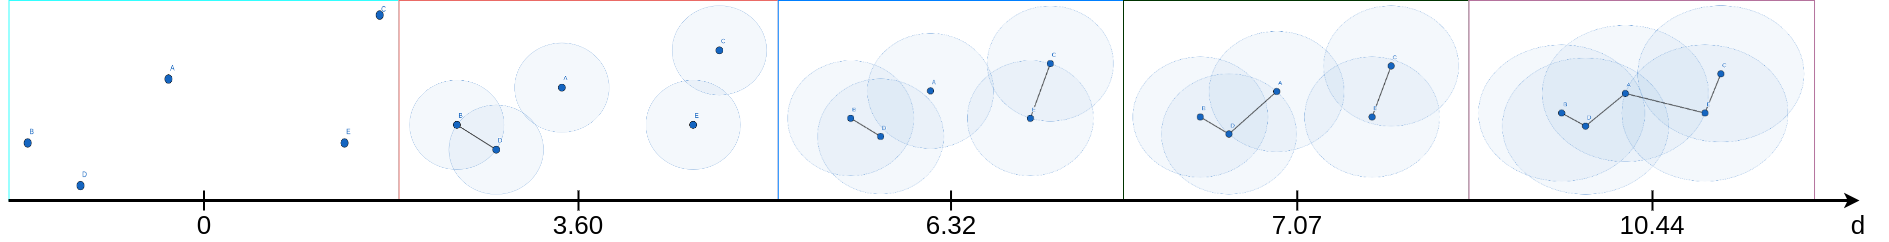
\includegraphics[width=1\textwidth, trim={0cm, 0.0cm, 0.0cm, 0.0cm}]{figures/barcodes_generation_border.png}\hfill
		%\hspace{-15mm}
		\subcaption{Vietoris-Rips filtration on FCN with the parameter $\epsilon$}
	\end{subfigure}
	\hfill
	\begin{subfigure}[t]{1\textwidth}
		\centering
		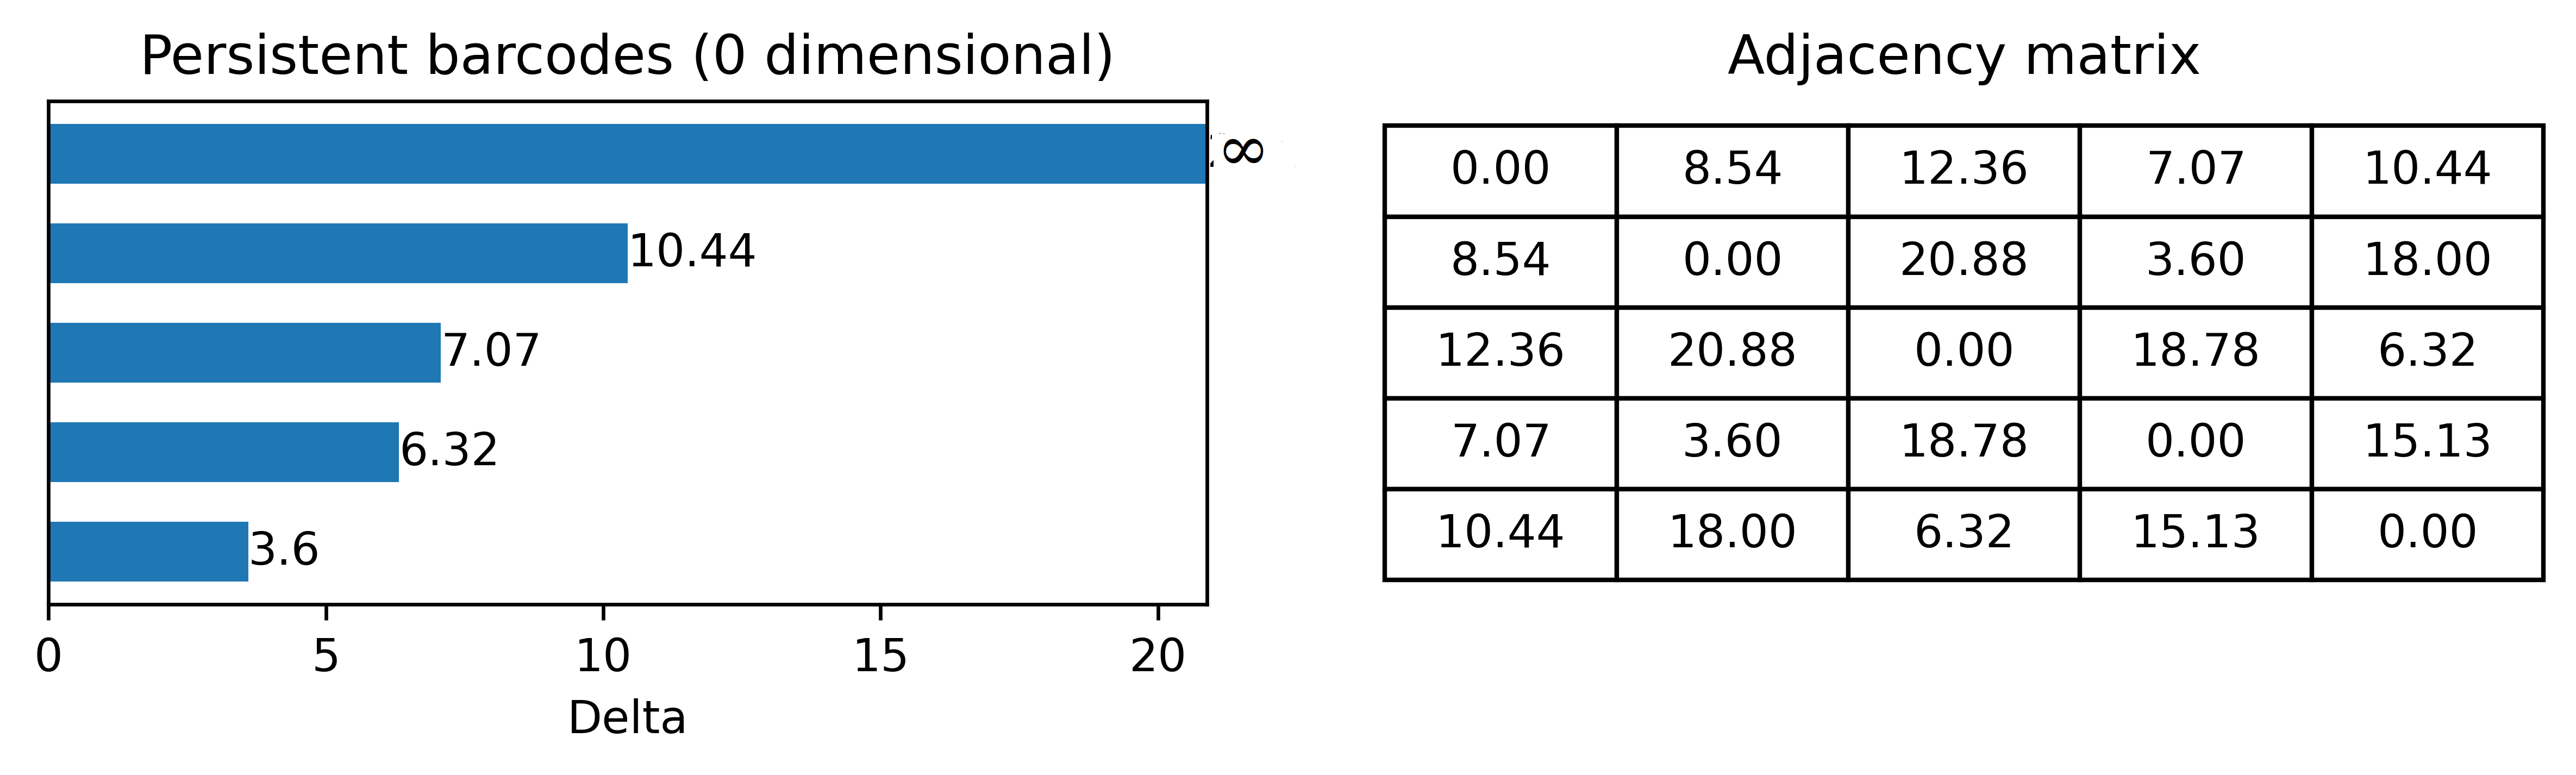
\includegraphics[width=1\textwidth, trim={0cm, 0.0cm, 0.0cm, 0.0cm}]{figures/barcode_matrix_title.png}\hfill
		%\hspace{-15mm}
		\subcaption{0-dimensional persistent barcodes (left) and adjacency matrix of the FCN (right)}
	\end{subfigure}
	\hfill
	\caption{An example of persistent homology to extract topological features using 0-dimensional barcodes. The adjacency matrix is of size $5 \times 5$.}
	\label{fig:rips_new}
\end{figure}
Persistent homology permits analysing a range of thresholds to gather connectivity information from FCN. Figure~\ref{fig:rips_new} shows an example of using persistent homology to record the changes of topological features over the changes of distances using zero-dimensional barcodes. Vietoris-Rips filtration on the given $5 x 5$ FCN is applied to capture the changes in the number of connected components for different parameters of $d$. We use an identical technique to capture topological features from fMRI FCNs extracted using different data acquisition parameters such as three different temporal sampling periods (2500ms, 1400ms, 645ms). We developed TDA based pipeline to illustrate the similarity of the extracted FCNs using the different temporal sampling periods. The TDA pipeline is formed mainly in three steps. First, we create FCNs from rs-fMRI data. Then we extract the persistent barcodes from the FCNs. Finally, we apply statistical analysis to show the similarity between extracted FCNs. This work aims to illustrate the potency of using persistent homology in capturing useful facts from fMRI datasets, proving the PH technique's resiliency towards the data acquisition parameters. To ensure the resiliency of the TDA pipeline, we also developed a nonTDA pipeline using the correlation coefficients of the fMRI datasets. 

Our TDA pipeline has the following steps:

\begin{enumerate}
    \item \textbf{Generate FCNs from rs-fMRI data}: We applied Pearson correlation on the fMRI dataset to generate the FCNs on different data acquisition parameters (2500ms, 1400ms, 645ms) as a data pre-processing step (Section~\ref{sec:fmri_to_fcn}).
    \item \textbf{Create distance matrix from FCNs}: The extracted FCNs are then converted into distance matrices as a weighted graph representing the correlation between time periods (Section~\ref{sec:fcn_to_ms}).
    \item \textbf{Extract persistent barcodes from distance matrix}: In this step, we extract persistent diagrams (0-dimensional barcodes) from the distance matrices using persistent homology to identify the topological features from the correlated matrices (Section~\ref{sec:ms_to_pd}).
    \item \textbf{Statistical analysis on PD to prove the resiliency of different data acquisition parameters}: Finally, we apply statistical analysis on the extracted barcodes to see the similarity between the topological features extracted using different data acquisition parameters (Section~\ref{sec:si}).
\end{enumerate}


\begin{figure}[H]%[!htb]
	\centering	
	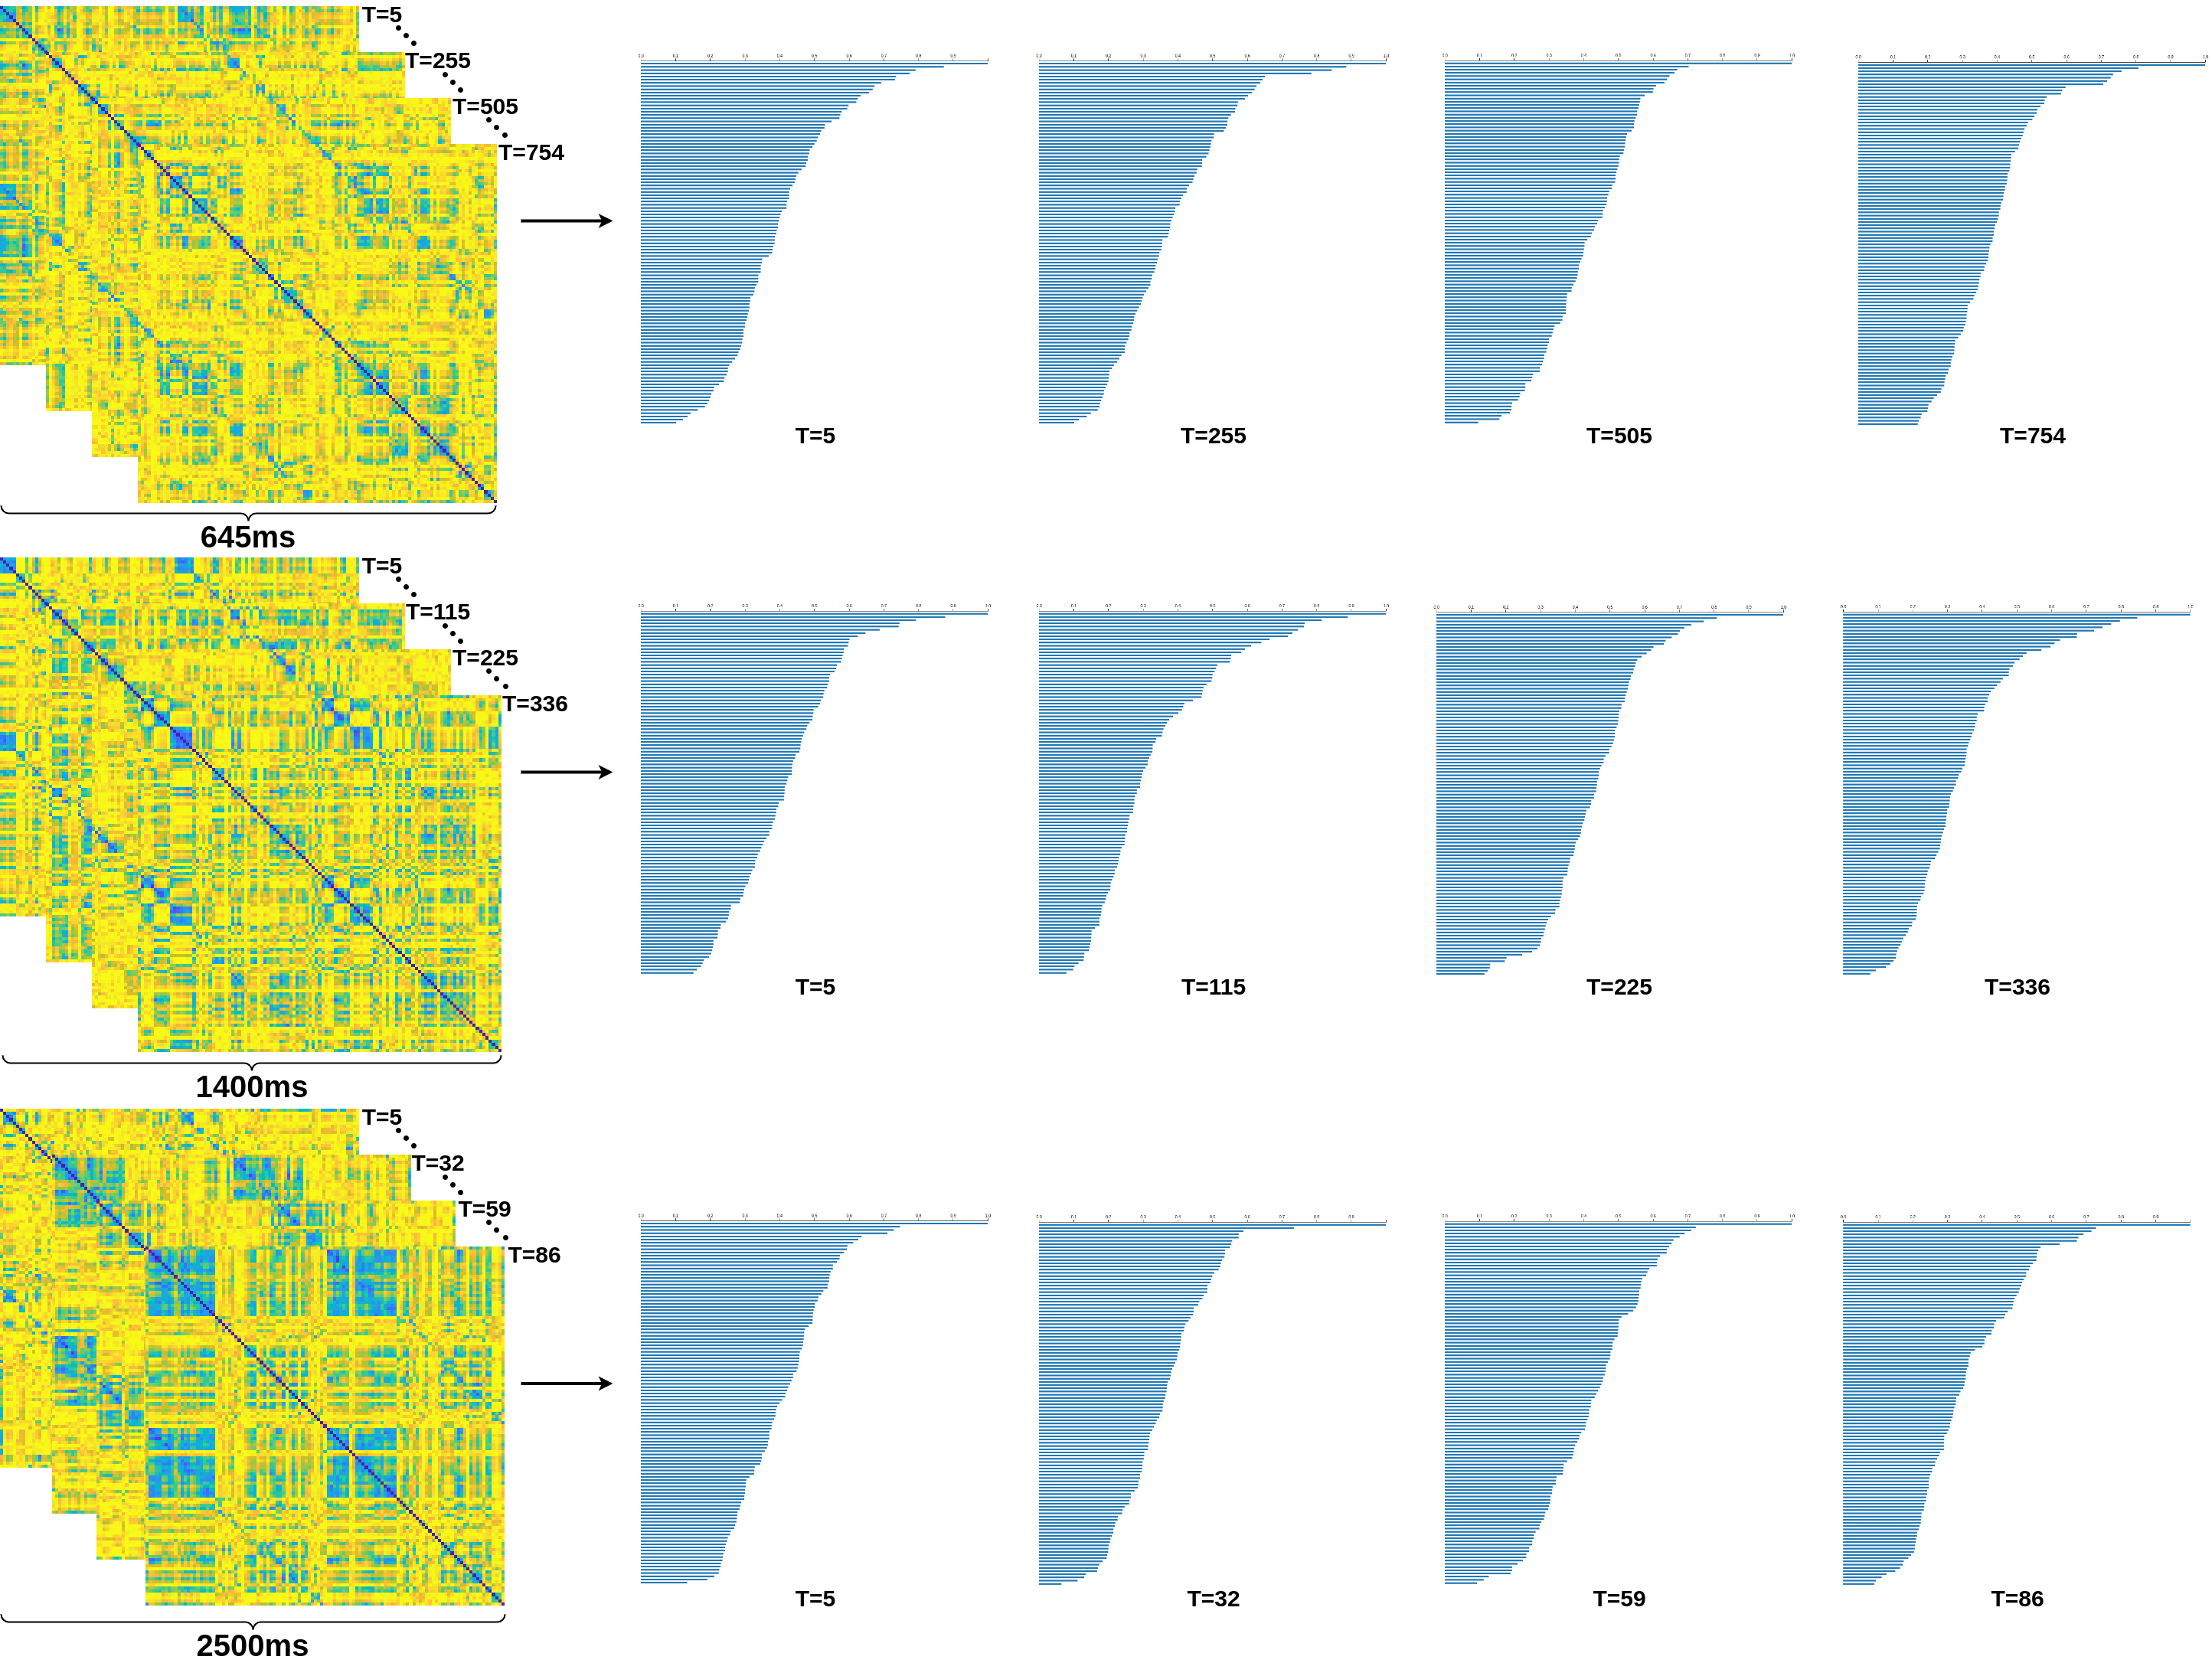
\includegraphics[width=1\textwidth, trim={0cm, 0.0cm, 0.0cm, 0.0cm}]{figures/stacked.png}
	\caption{The FCN and extracted topological feature as 0-dimensional barcodes for subject $32$ at different time points for temporal sampling periods $645ms$ (top), $1400ms$ (center), and $2500ms$ (bottom). The matrix size is $113 \times 113$.}
	\label{fig:wd1}
\end{figure}

\subsection{FCN generation from fMRI data}
\label{sec:fmri_to_fcn}
\textcolor{red}{
Structural T1-weighted and rs-fMRI data were obtained from the openly available Enhanced Nathan Kline Institute Rockland Sample database (NKI-RS)~\cite{nooner2012nki}. 
The MRI data were obtained using a 3T Siemens Magnetom Tim Trio scanner. 
The data acquisition parameters for the T1-weighted structural data were: $1.0$ mm isotropic voxels with 176 slices, 
repetition time (TR) = $1900$ ms,
echo time (TE) = $2.52$ ms and field of view (FOV) = $250 \times 250$.
Resting state fMRI data were acquired using multiband echo-planar imaging (EPI)~\cite{feinberg2010multiplexed} from each subject using three different acquisition protocols with different parameters as follows. 
(1) $3.0$ mm isotropic voxels with $40$ slices, \emph{TR = 645 ms}, TE = $30$ ms, FOV = $222 \times 222$ mm, number of volumes = $900$, andmulti-band factor = $4$.
(2) $2.0$ mm isotropic voxels with $64$ silces, \emph{TR = 1400 ms}, TE = $30$ ms, FOC = $224 \times 224$ mm, number of volumes = $404$ and multi-band factor = $4$. (3)
$2.0$ mm isotropic voxels with 38 slices, \emph{TR = 2500 ms}, TE = $30$ ms; FOV = $216 \times 216$ mm, number of volumes = $120$ and multi-band factor = $1$.
It can be seen that even though we identify the three datasets from each subject with the corresponding TR, the data differ in many other scan parameters such as number of volumes, multiband factor, FOV and voxel size.
}

\textcolor{red}{
The MRI data were subjected to a standard pre-processing pipeline, including the first five volume removal, slice time correction and motion correction. T1-weighted anatomical images were coregistered to the mean functional images, using which the fMRI images were spatially registered to a standard MNI152 template. Nuisance variables such as low-frequency drifts and motion parameters were regressed out. Unwanted physiological fluctuations (white-matter and cerebrospinal fluid signals) were removed using aCOMPCor (anatomical component-based noise correction). After removing subjects that failed quality control, 316 subjects were identified to have usable data from all three acquisition protocols. Subsequently, mean time series from 113 brain regions (obtained using the Yeo parcellation template ~\cite{thomas2011organization}) were obtained for each subject and acquisition protocol.
Using Pearson’s correlation, FCN matrices were estimated from these mean time series. 
}

At this stage, we generate one FCN for each fMRI scan. Each FCN is stored as a symmetric adjacency matrix $M$ with size $113 \times 113$, where $M_{ij}$ represents the correlation coefficient between brain nodes $i$ and $j$. The dataset consists of three temporal frequencies ($645$ms, $1400$ms and $2500$ms). There are $316$ subjects for each temporal frequency. The $2500$ms temporal frequency has 86 timesteps, $1400$ms has 336 timesteps, and $645$ms has 754 timesteps. The total number of adjacency matrices is $371,616$ $(316 \times 86) + (316 \times 336) + (316 \times 754)$ with a dimension of $113 \times 113$. Figure~\ref{fig:wd1} shows an example of the FCN for subject $31$, for the three sampling periods ($645$ms, $1400$ms and $2500$ms).


\subsection{Creation of matrices from FCNs}
\label{sec:fcn_to_ms}

Usually, topological data analysis uses point cloud data in metric configuration. We confine the weighted networks from fMRI data in distance matrices in our TDA pipeline before applying TDA techniques. Then, we extract persistent barcodes from the distance matrices. 


We use popular Pearson’s correlation coefficients $pcc(p_t, q_t)$ to measure the interrelation between any two data points (nodes) $p_t$ and $q_t$ at time $t$ in the fMRI data as it is independent on FCN construction method ~\cite{smith2011network}. This technique ensures that to map of the higher correlations between the data points to a smaller value. The mapping for the distance matrix calculation is:

\[
\mathit{d(p_t, q_t)} = 
\sqrt{ 1 - pcc(p_t, q_t)^2 }
\]

The temporal indexing $t$ indicates this is a temporal dataset, and the correlations and distances are calculated between node pairs at each time point.

\subsection{Extract persistent barcodes from distance matrix}
\label{sec:ms_to_pd}

Using persistent homology, we capture topological features from the distance matrices extracted from the fMRI FCNs. This section overviews topological feature extraction using persistent barcodes and the distance metric we have used. The existing literature contains the details on these topics ~\cite{edelsbrunner2008surveys, Topology_and_data}.

\subsubsection{Extraction of topological features using persistent homology}

Persistent homology can extract topological features from a topological space. The homology of the space can be divided into groups based on the dimensions of the features. A topological space $\mathbb{X}$ can be divided into homology groups $H_i(\mathbb{X})$ for $i={0, 1, 2, ...}$ where $H_i(\mathbb{X})$ represents the $i^th$ homology group. Each homology group $H_n(\mathbb{X})$ denotes the number of n-dimensional holes in the topological space $\mathbb{X}$. For example, the $H_0(\mathbb{X})$ homology group shows the number of connected components, $H_1(\mathbb{X})$ homology group shows the number of holes, $H_2(\mathbb{X})$ homology group shows the number of voids in the topological space $\mathbb{X}$. 

In this paper, we use $H_0(\mathbb{X})$ homology group (0-dimensional) to extract the number of connected components from the rs-fMRI FCNs as topological features. Figure \ref{fig:rips_new} shows a simple example of using persistent homology to extract the topological features from a given FCN. The table at the bottom right in Figure \ref{fig:rips_new}(b) represents the adjacency matrix of an FCN with five nodes. Persistent homology captures the changes in topological features over distance thresholds ($\epsilon$) between the nodes. In a point cloud, $F$ with $p$ nodes, two nodes ($x$, $y$) are marked as connected with an edge if the distance $d(x, y)$ is less than threshold $\epsilon$. In this scenario, they form a 1-Simplex. When three nodes are connected with each other for some value of $\epsilon$, they form 2-Simplex and so on. For a given $\epsilon$, the graph is called a Rips complex represented by $Rips(F , \epsilon)$. These continuous changes in the value of $\epsilon$ result in the changes in topological features. Vietoris-Rips filtration captures the increasing value of $\epsilon$ for which a new Rips-complex, in another word, new topological feature, is being generated \cite{bauer2021ripser}. Figure \ref{fig:rips_new}(a) shows the extraction of different topological features in various thresholds of $\epsilon$ using Vietoris-Rips filtration. 

For each real number $t$ where topological features are changed, we consider them important events and store these values of $t$. For instance, at some time $t_0$, a topological feature, a component is being created, and at time $t_1$, it is merged with another component. We keep track of the $birth$ as $t_{birth} = t_0$ and $death$ as $t_{death} = t_1$ for each component. The time of the $(t_{birth}, t_{death})$ of the topological features is visualized as $barcodes$. The span of time for each feature $t_{death} - t_{birth}$ is called as persistence of that feature. Figure \ref{fig:rips_new}(b)(left) shows the barcodes for the given FCN. At $t=0$, five topological features are born as five independent (connected) components. At $t=3.6$, two components are merged; thus, the death of a component is recorded at $t=3.6$. Therefore, the persistence of that component is $3.6$. Similarly, at $t=6.32$, another component is merged with a persistence of $6.32$. For 0-dimensional persistence barcodes, this process continues until there is only one connected component. This last component never dies; thus, the persistence of this component is $\infty$. The 0-dimensional persistence barcodes in Figure \ref{fig:rips_new}(b)(left) represent the $birth$ and $death$ of the topological features, which is the changes in the number of connected components of the FCN. Each horizontal bar begins at the birth of a component and ends at the death of each component in the barcodes representation. 

In our pipeline, we generate 0-dimensional persistent barcodes for each FCN. Each FCN has $113$ vertices that form the finite set of points $F$ where the value $d_i$ represents the pairwise distance between the points. We extract 0-dimensional barcodes using persistent homology for all the $371,616$ FCNs $((316 \times 86) + (316 \times 336) + (316 \times 754))$. An illustration of the extracted barcodes at $timestep=1$ for all three temporal sampling periods ($645ms$, $1400ms$, $2500ms$) for a single subject is shown in Figure \ref{fig:wd1}.


\subsection{Statistical analysis}
\label{sec:si}

A persistent barcode can be represented with a persistent diagram without information loss where the birth and death of a component (a topological feature) are represented as a point on the X-axis and Y-axis, respectively. These points on a two-dimensional surface as a \emph{persistent diagram} can be used for statistical inference to prove that persistent homology is resilient to different data acquisition parameters. The literature shows the usability of earth moving distance, also known as Wasserstein distance (WD), for statistical inference of persistent diagrams \cite{vallender1974calculation, edelsbrunner2013persistent}.

We use WD as a metric to compute the distance between two persistence diagrams extracted from two FCNs. WD represents the minimum value that is computed in the match calculation between the points of two persistent diagrams. The WD value of two similar persistent diagrams is smaller than two dissimilar persistent diagrams. This WD metric assists in proving the hypothesis of similarity between the persistent diagrams extracted from different data acquisition parameters, such as sampling rates. 

We develop two frameworks for statistical analysis: (a) topological data analysis framework and (b) traditional FCN analysis framework. We used Matlab during the data preprocessing steps and Python for statistical analysis. For the topological data analysis framework, we used \emph{Gudhi} library~\cite{jea_hera} to compute the 0-dimensional barcodes from FCNs and to calculate WD distances between the persistent diagrams. We also used \emph{scikit-learn} library for multidimensional scaling, and cluster calculation \cite{scikit-learn}.

\subsubsection{Topological data analysis framework}
\label{sec:tda_pipeline}



We develop a topological data analysis (TDA) framework to test our hypothesis of the similarity of the fMRI FCNs on different data acquisition parameters, such as different temporal sampling rates (TR). Our dataset includes three data cohorts: $645ms$, $1400ms$, and $2500ms$. For these TRs, each of the subjects (316 in total) has 754, 336, and 86 timesteps, respectively. Figure \ref{fig:tda_pipeline} represents the TDA pipeline we develop for the TDA framework. We calculate pairwise WD between the persistent diagrams of the timesteps for all subjects within the same data cohort. 

Let,
\begin{align*}
S_i & = \text{Subject } i, \text{ where } i = 1,2,\ldots,316 \\
T_k & = \text{Number of time steps for data cohort } k, 
\\
& \text{ where } k\in(645ms, 1400ms, 2500ms) \\
P_{S_i,t} & = \text{Persistence diagram for subject } S_i \text{ at time } t \\
d_W(P_1,P_2) & = \text{Wasserstein distance between persistence diagrams } P_1 \text{ and } P_2
\end{align*}

The TDA distance matrix for a given subject $S_i$ in cohort $k$ is defined as:
\begin{equation}
D(S_i)_{t_1,t_2} = d_W(P_{S_i,t_1}, P_{S_i,t_2}) \quad \text{for } t_1, t_2 = 1, \ldots, T_k \label{eq:tda_dis}
\end{equation}

In Eq. \ref{eq:tda_dis}, we compute the pairwise Wasserstein distance between persistence diagrams at times $t_1$ and $t_2$ which gives a $T_k \times T_k$ distance matrix for each subject $S_i$. We have three data cohorts ($645ms$, $1400ms$, $2500ms$) with different timesteps (754, 336, 86). Thus, we get 316 adjacency matrices for each data cohort with size ($754 \times 754$), ($336 \times 336$), and ($86 \times 86$), respectively.

\begin{figure}[H]%[!htb]
	\centering	
	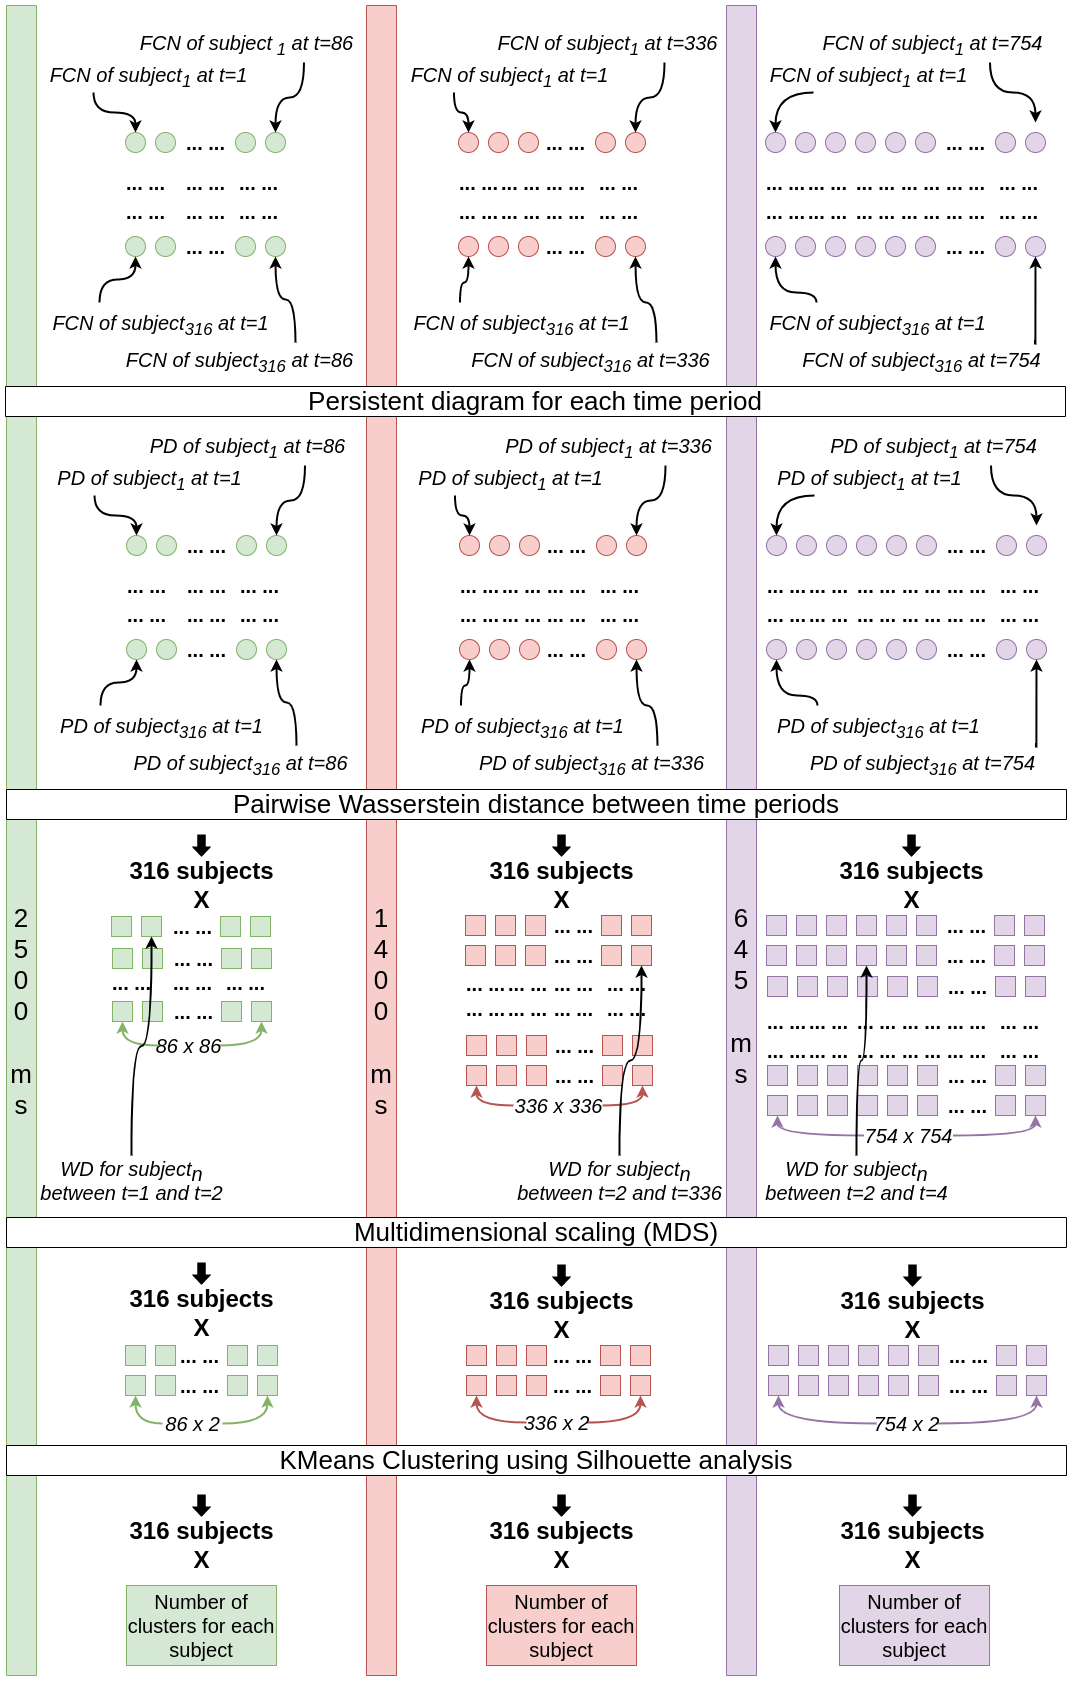
\includegraphics[width=0.9\textwidth, trim={0cm, 0.0cm, 0.0cm, 0.0cm}]{figures/tda_pipeline.png}
	\caption{TDA pipeline.}
	\label{fig:tda_pipeline}
\end{figure}

These high dimensional adjacency matrices are complex to analyze by statistical methods. To make it interpretable by the statistical methods, We apply two component multidimensional scaling (MDS) technique to reduce the dimensionality of the matrices. After this stage, we get 316 adjacency matrices for each data cohort with size ($ 754 \times 2 $), ($ 336 \times 2 $), and ($ 86 \times 2 $). The two-dimensional MDS results are plotted using scatter plots that give an intuition to use clustering to calculate the similarity between the TRs. We apply the k-means clustering technique to the MDS results to get the number of clusters for the reduced-sized matrices. As k-means clustering requires configuring the number of clusters $n$ before the cluster computation, we choose $n$ using a well-known approach called Silhouette analysis. Using Silhouette analysis, we choose $n$ that gives the maximum Silhouette score for the given adjacency matrices between the range from 2 to 16 \cite{scikit-learn, rousseeuw1987silhouettes}. After calculating the number of clusters for all three data cohorts, we get the number of clusters for all 316 subjects across these data cohorts. A similar number of clusters for the same subject across three data cohorts will indicate the similarity between the subjects for different data acquisition parameters (different TRs in our case). If we get significant similarity between the TRs, we can conclude the resiliency of persistent homology for rs-fMRI data analysis with different data acquisition parameters.



\subsubsection{Traditional FCN analysis}
\label{sec:nontda_pipeline}
Alongside the TDA framework, we also develop a nonTDA framework to show the efficiency of persistent homology over the traditional FCN analysis for the rs-fMRI dataset with different temporal sampling periods. The nonTDA framework is illustrated in Figure \ref{fig:nontda_pipeline}. Instead of the persistent diagrams or applying any persistent homology methods, we use a correlation coefficient between the timesteps for all three data cohorts. 
\begin{figure}[H]%[!htb]
	\centering	
	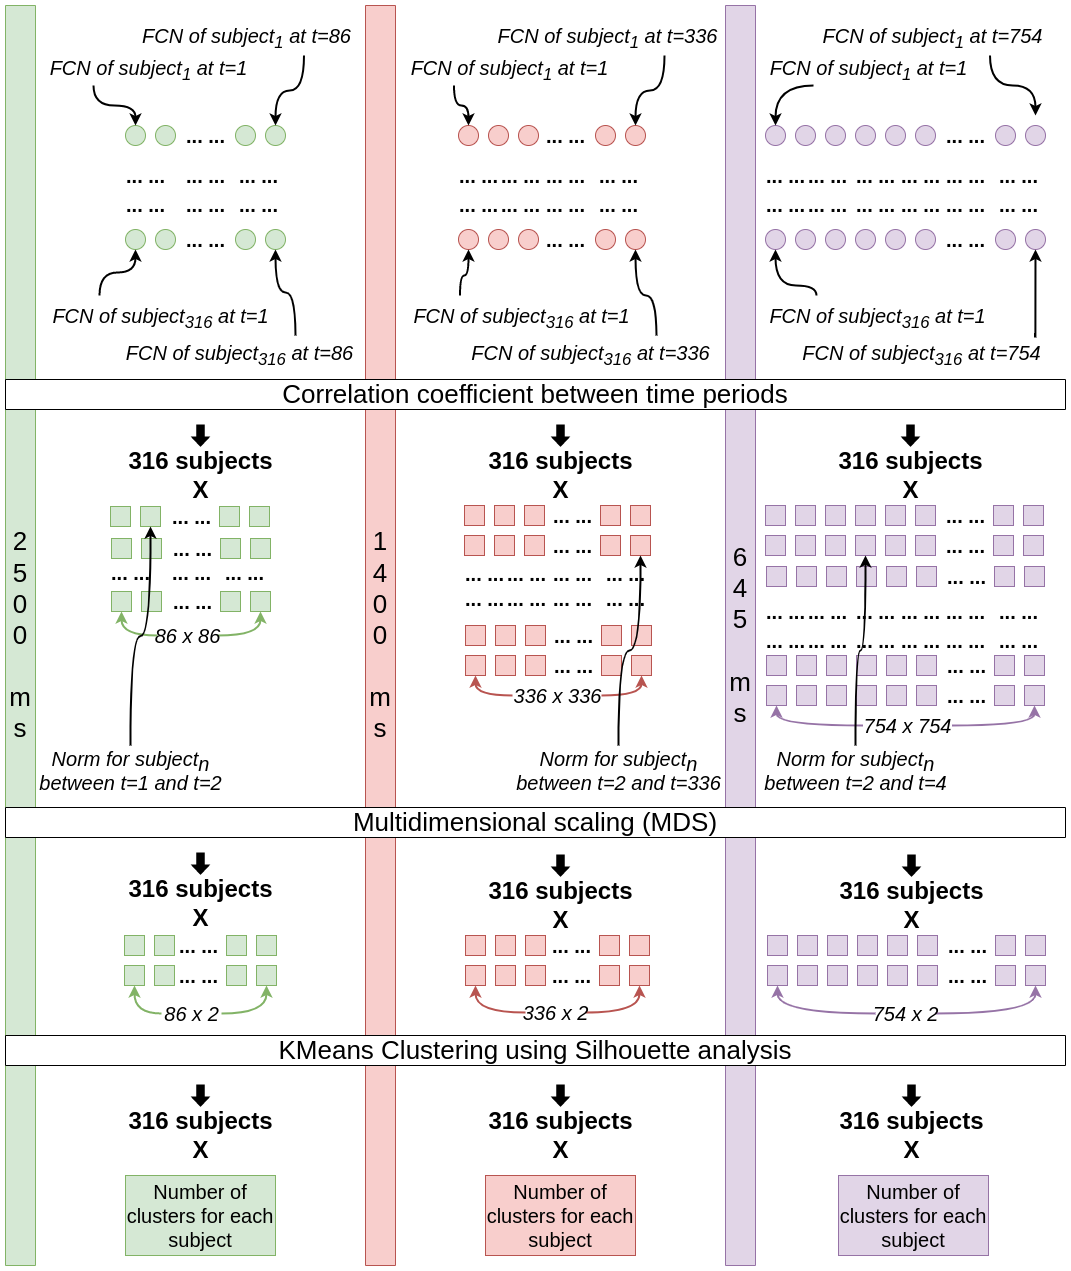
\includegraphics[width=0.9\textwidth, trim={0cm, 0.0cm, 0.0cm, 0.0cm}]{figures/non_tda_pipeline.png}
	\caption{Non TDA pipeline}
	\label{fig:nontda_pipeline}
\end{figure}

Let,
\begin{align*}
S_i &= \text{Subject } i, \text{ where } i = 1,2,\ldots,316 \\
T_k &= \text{Number of time steps for data cohort } k, \\
&\text{ where } k\in(645\text{ms}, 1400\text{ms}, 2500\text{ms}) \\
A_{S_i,t} &= \text{Adjacency matrix for subject } S_i \text{ at time } t
\end{align*}

The distance matrix for a given subject $S_i$ in cohort $k$ is defined as:

\begin{equation}
D(S_i)_{t_1,t_2} = \sqrt{\sum_{m=1}^{M} \sum_{n=1}^{N} |a_{mn}^{t_1} - a_{mn}^{t_2}|^2}
\label{eq:nontda_dis}
\end{equation}

In Eq. \ref{eq:nontda_dis}, $M, N$ are the dimensions of the adjacency matrices. We compute the Eucledean distance between adjacency matrices at times $t_1$ and $t_2$ which gives 316 distance matrices of sizes ($86 \times 86$), ($336 \times 336$), and ($754 \times 754$) for the three cohorts respectively. In this stage, we acquire 316 matrices for each of the data cohorts with the size of ($86 \times 86$) for $2500ms$,  ($336 \times 336$) for $1400ms$, and ($754 \times 754$) for $645ms$. Then we follow a similar pipeline of the TDA framework to keep the comparison uniform. We reduce the dimension of the matrices using two-component multidimensional scaling (MDS) and then calculate the number of clusters ($n$) on the reduced matrices using k-means clustering. We also use the maximum Silhouette score to choose the value of $n$ within the range from 2 to 16. Finally, this pipeline will also produce the number of clusters of the MDS for every 316 subjects for all three data cohorts. Our hypothesis will be proven right if the TDA pipeline gives a better similarity score than the nonTDA pipeline. 
\begin{figure}[!ht]%[!htb]
	\centering
	\begin{subfigure}[!ht]{1\textwidth}
		\centering
		\hspace{8mm}
		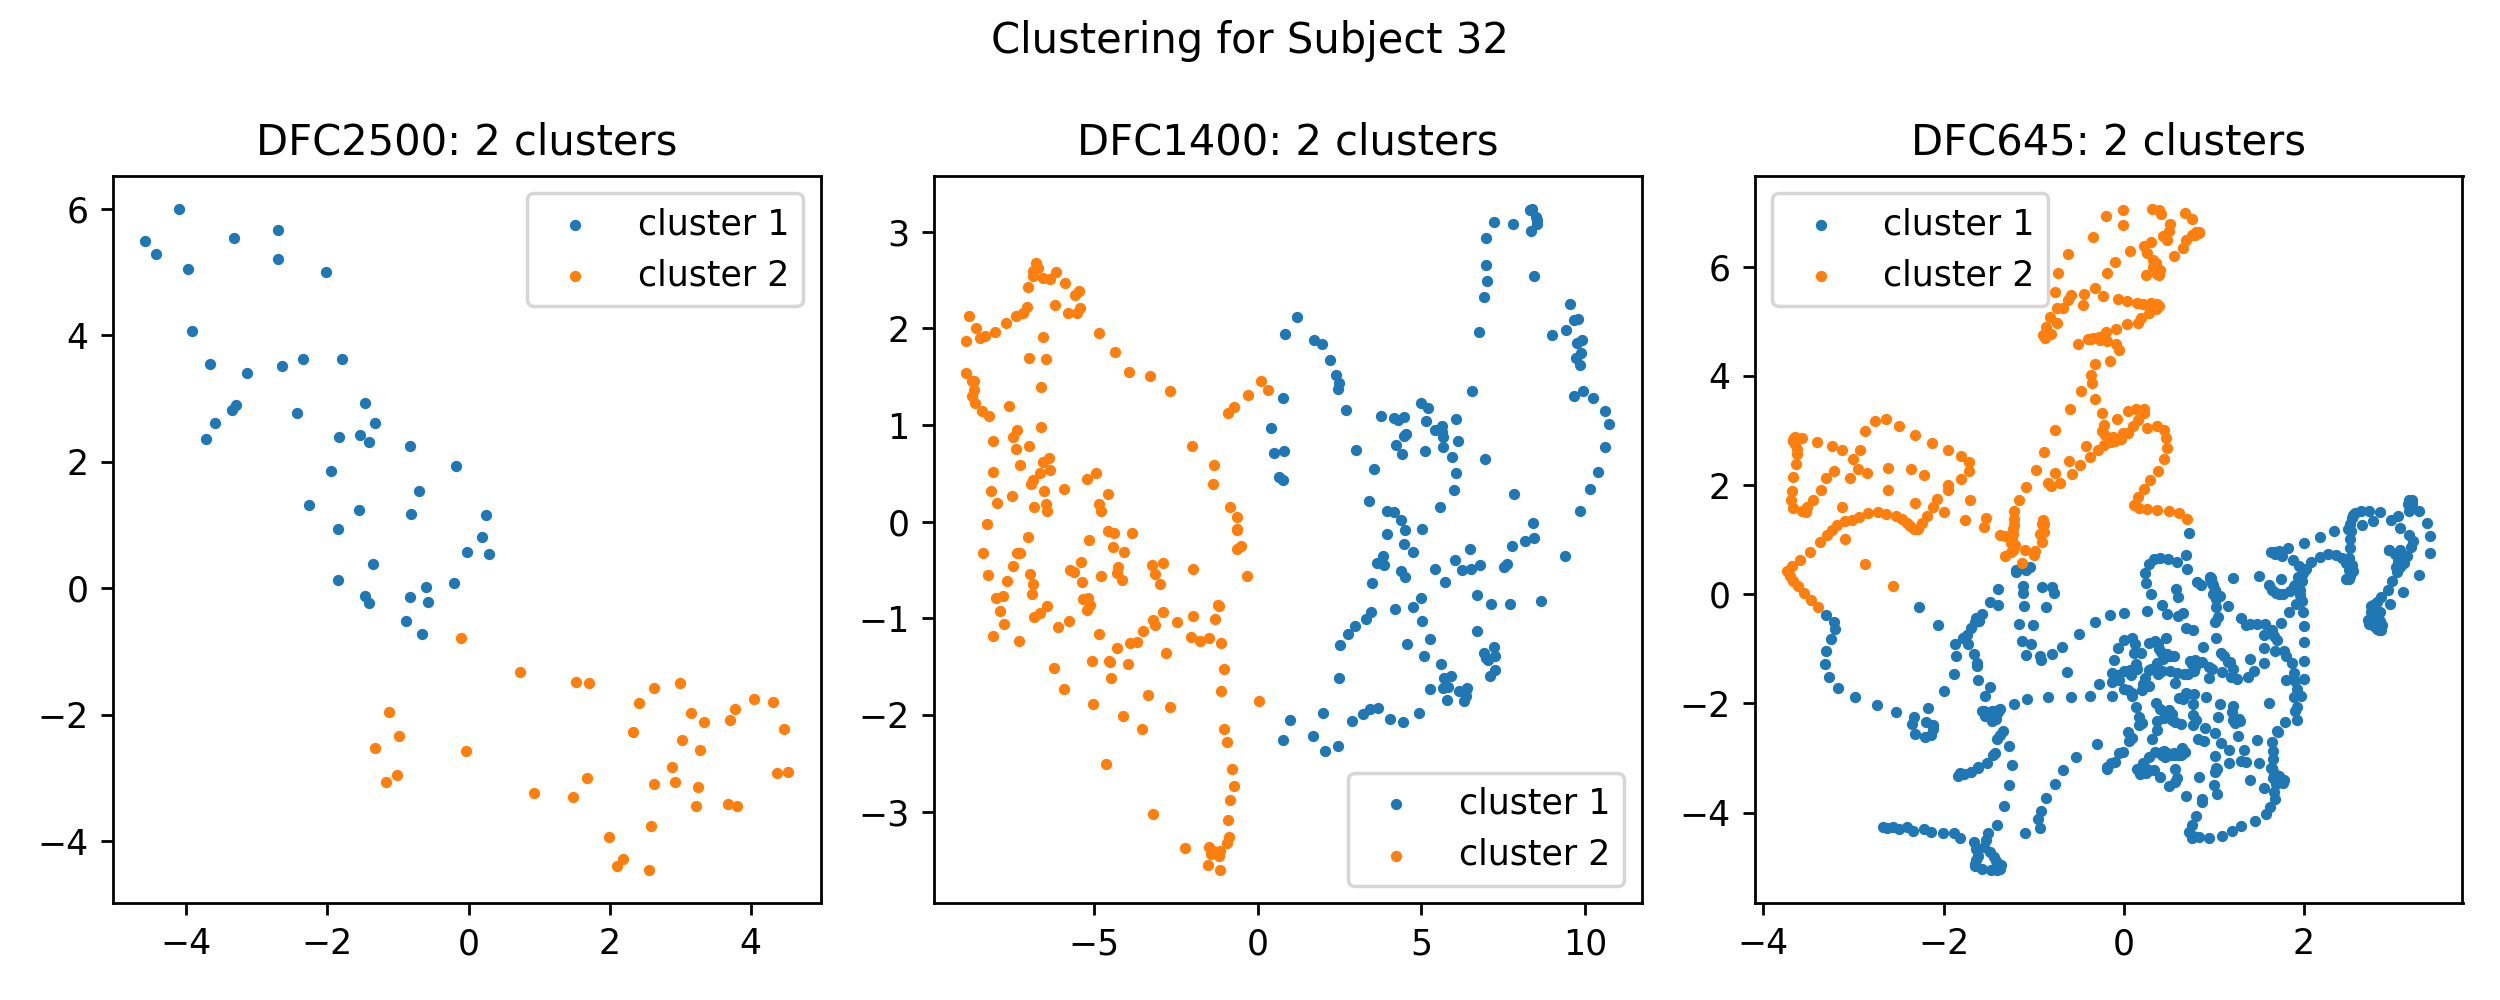
\includegraphics[width=1\textwidth, trim={0cm, 0.0cm, 0.0cm, 0.0cm}]{figures/clusters/subject_32.png}\hfill
	\end{subfigure}
	\begin{subfigure}[!ht]{1\textwidth}
		\centering
		\hspace{8mm}
		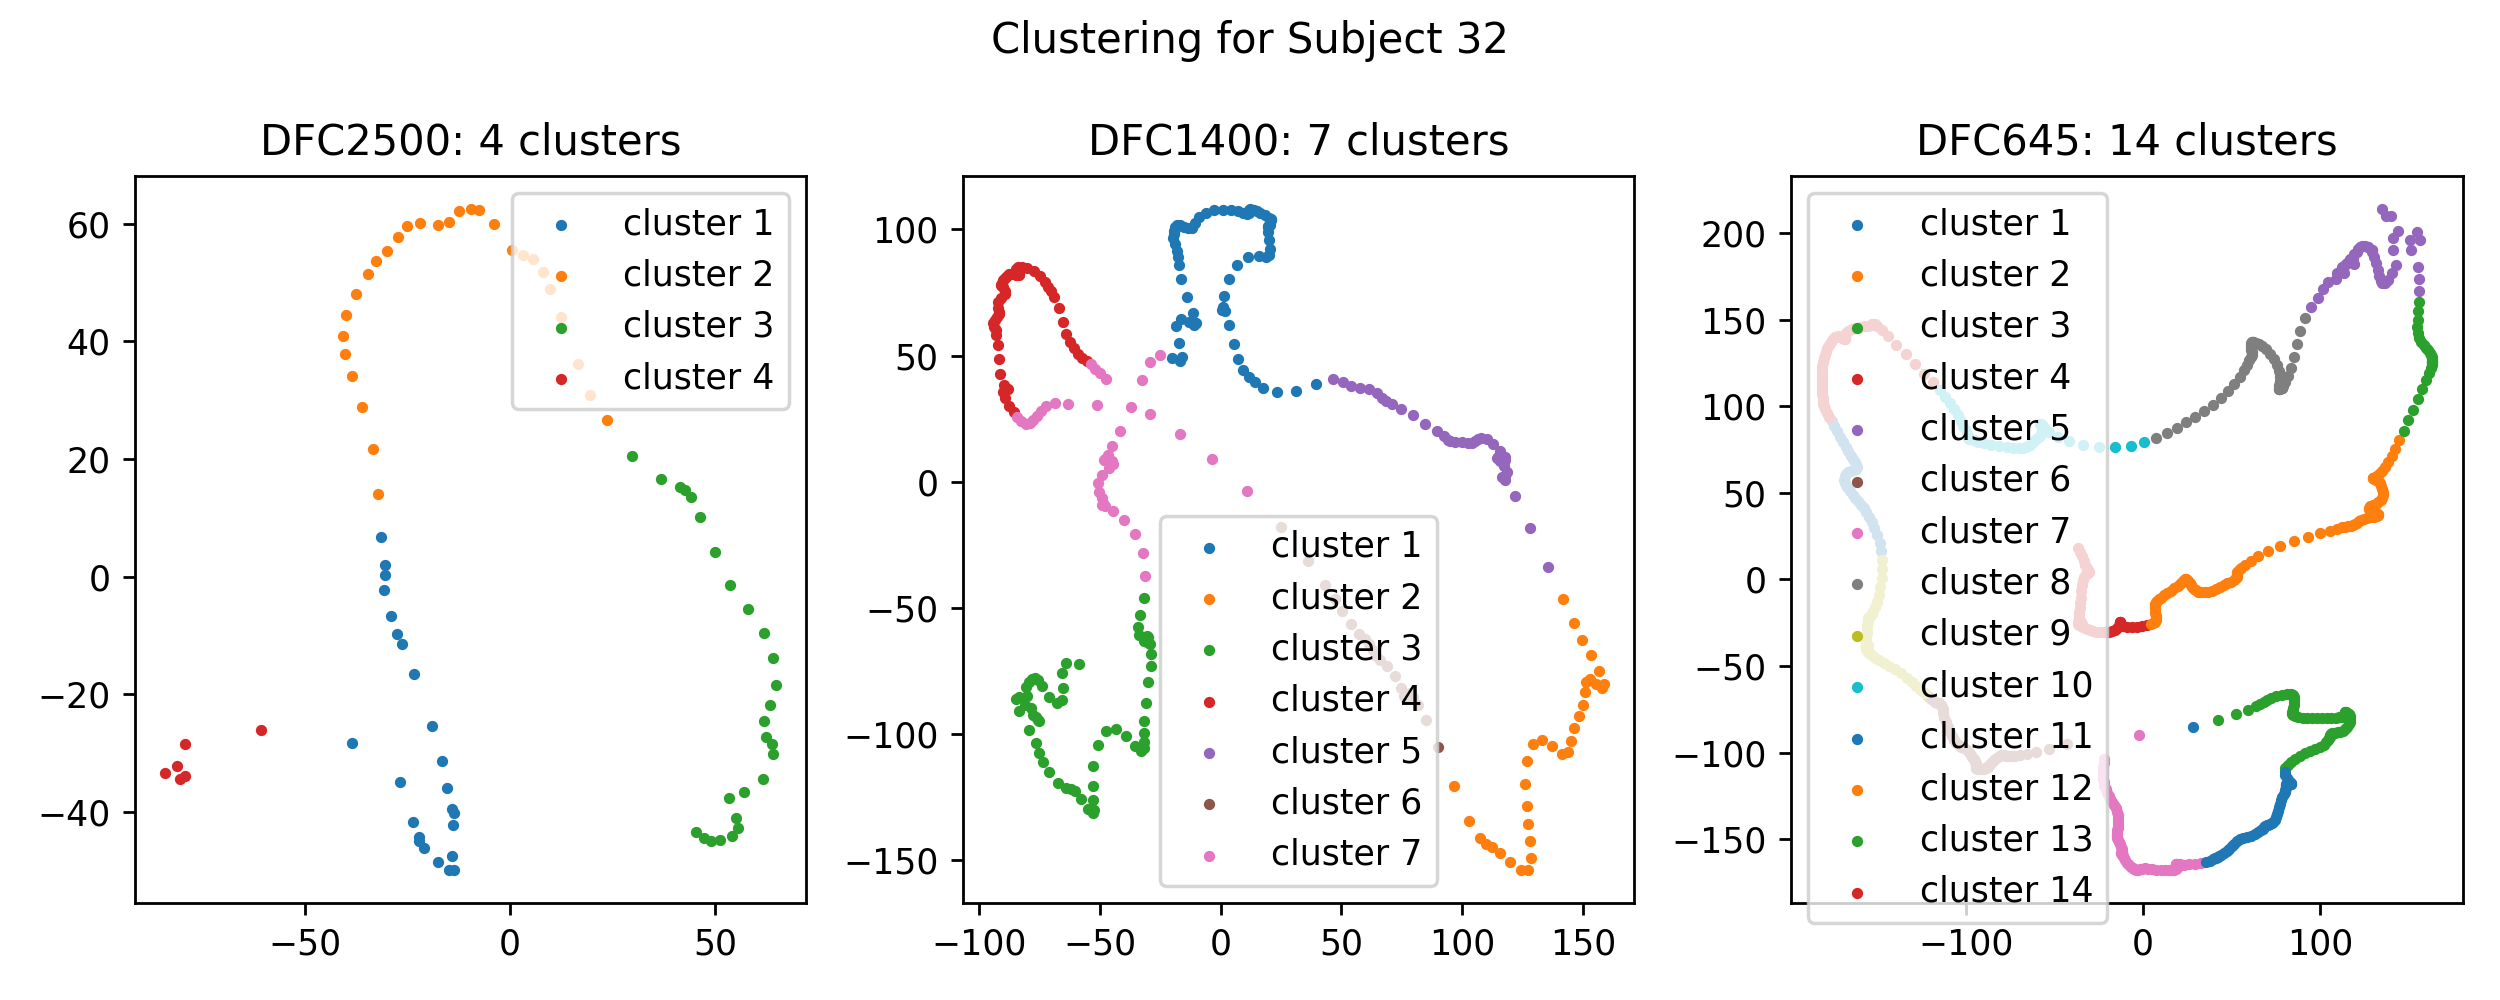
\includegraphics[width=1\textwidth, trim={0cm, 0.0cm, 0.0cm, 0.0cm}]{figures/clusters/subject_32_non_tda.png}\hfill
	\end{subfigure}
	\caption{Clustering result for subject $32$ (top row) for temporal period $2500ms$ (left), $1400ms$ (center), and $645ms$ (right). Clustering result for the same subject (bottom row) with NonTDA Clustering result.}
	\label{fig:clus}
\end{figure}

\section{Results}
\label{sec:eval}
Our TDA and nonTDA pipelines start with embedding one FCN for each rs-fMRI scan as an adjacency matrix (section~\ref{sec:fmri_to_fcn}). In this stage, we get $371,616$ adjacency matrices ($(316 \times 86) + (316 \times 336) + (316 \times 754)$) for three temporal sampling periods ($2500ms$, $1400ms$, $645ms$). Each matrix has a dimension of $113 \times 113$. For example, the FCNs for the three sampling periods for subject $1$ are shown in Figure~\ref{fig:wd1}. In the second stage of the pipelines, we embed the FCN using Pearson's correlation coefficients and range the values between $0$ and $1$. The third stage of the TDA pipeline extracts 0-dimensional persistent barcodes from the matrices using persistent homology (section~\ref{sec:ms_to_pd}). The bottom row of Figure~\ref{fig:wd1} shows the extracted 0-dimensional barcodes for the three TRs. In the nonTDA pipeline, instead of using persistent homology, we used correlation coefficients between the timesteps for the three TRs. We continue to the statistical analysis phase, where we evaluate the resiliency of our TDA framework on different temporal sampling periods of rs-fMRI datasets (section~\ref{sec:si}).


\begin{figure}[!ht]
	\centering
	\begin{subfigure}[!ht]{1\linewidth}
		\centering
		\hspace{8mm}
		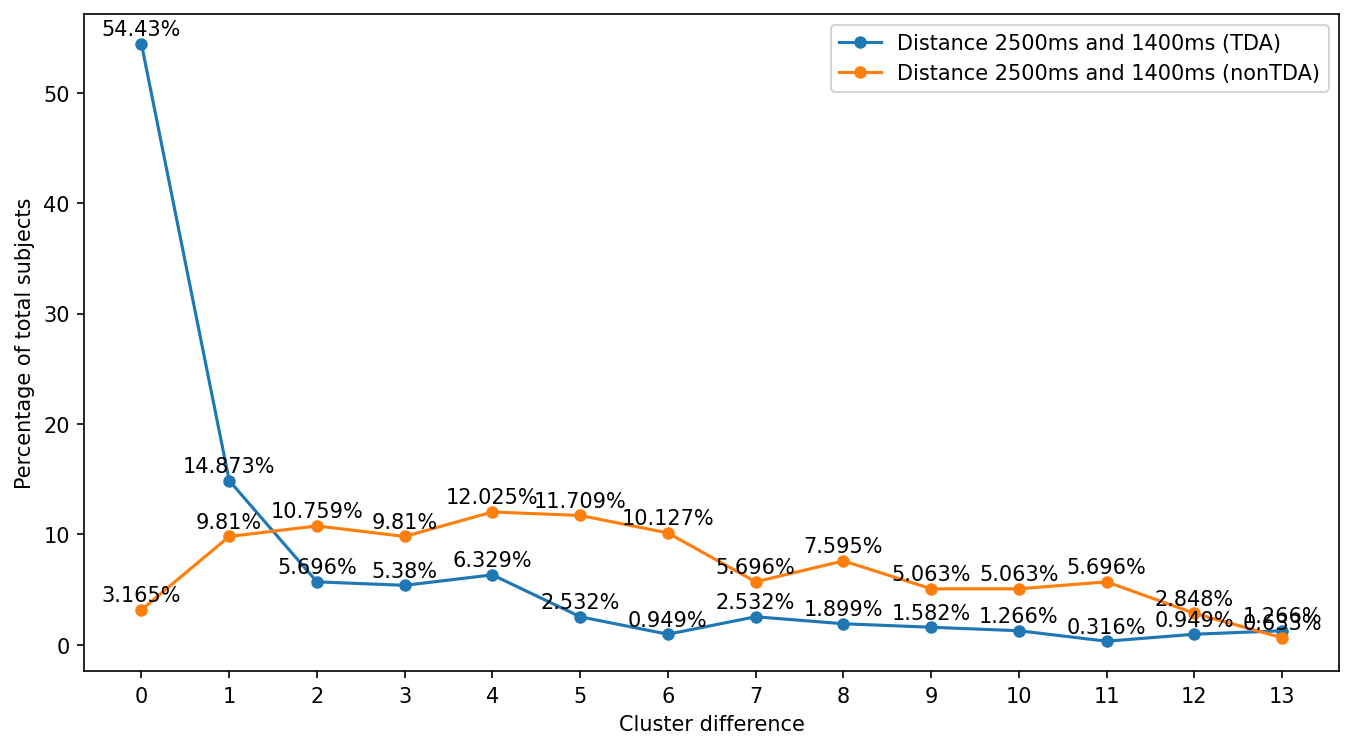
\includegraphics[width=0.8\textwidth, height=0.28\textheight]{figures/pairwise_2500_1400.png}\hfill
		%\hspace{-15mm}
	\end{subfigure}
	\begin{subfigure}[!ht]{1\linewidth}
		\centering
		\hspace{8mm}
		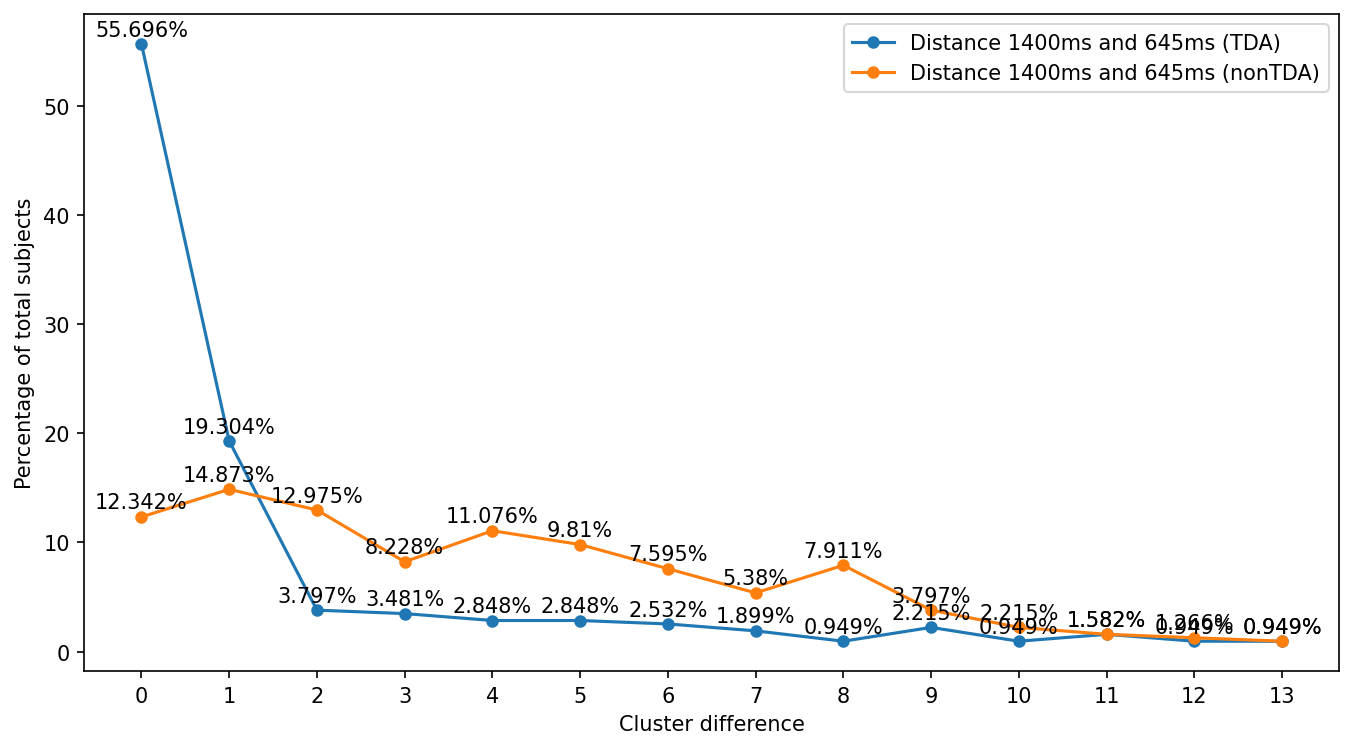
\includegraphics[width=0.8\textwidth, height=0.28\textheight]{figures/pairwise_1400_645.png}\hfill
		%\hspace{-15mm}
	\end{subfigure}
	\begin{subfigure}[!ht]{0.8\linewidth}
		\centering
		\hspace{8mm}
		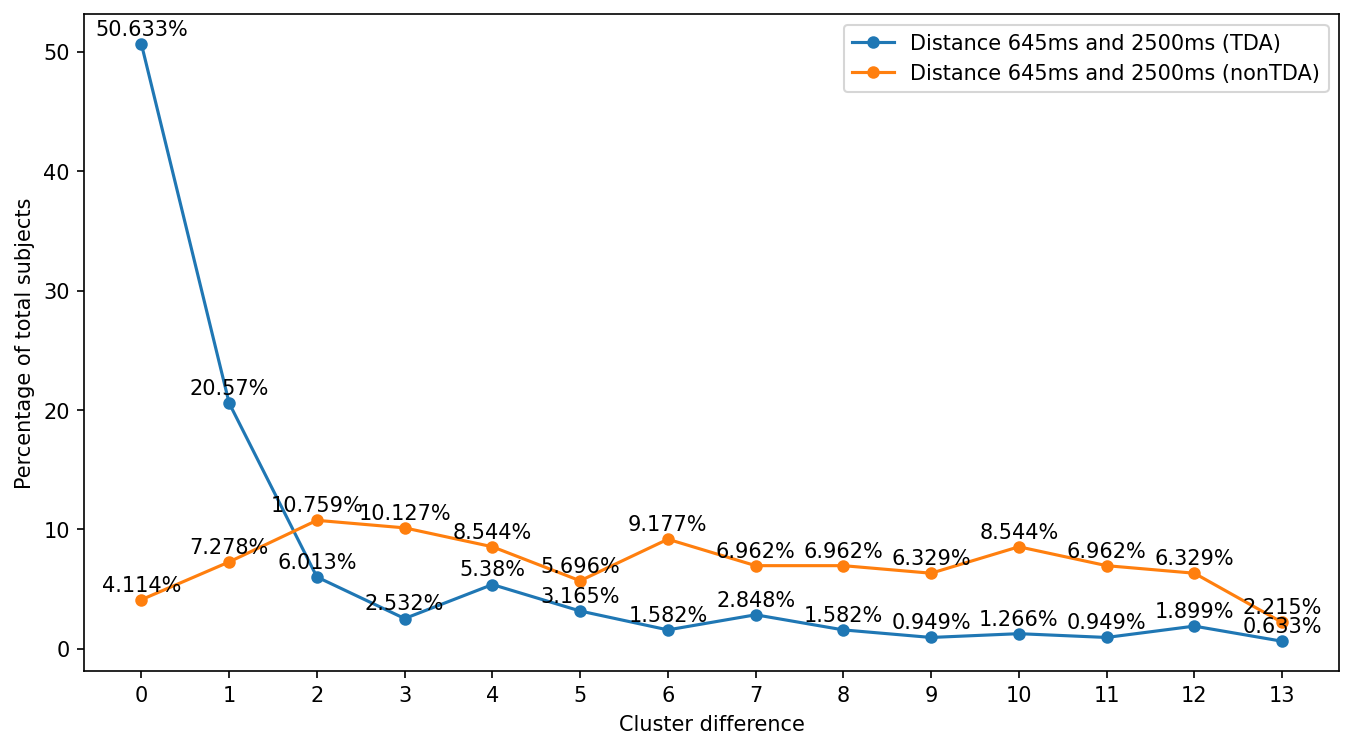
\includegraphics[width=1\textwidth, height=0.28\textheight]{figures/pairwise_645_2500.png}\hfill
		%\hspace{-15mm}
	\end{subfigure}
	\caption{Pairwise cluster distance comparison between TDA and nonTDA pipeline. Comparison between temporal sampling $2500$ and $1400$ (top row), temporal sampling $1400$ and $645$ for TDA and nonTDA pipeline(top row), temporal sampling $645$ and $2500$(bottom row)}
	\label{fig:clus_distance_pairwise}
\end{figure}

In the TDA pipeline, we use the Wasserstein distance metric on the persistent diagrams for all the subjects for all three temporal sampling periods. On the contrary, in the nonTDA pipeline, we directly use the correlation coefficient on the extracted FCNs. Adjacency matrices generated after this stage in both pipelines are similar in size for respective temporal sampling periods. For temporal sampling period $2500ms$ with $86$ timesteps in the TDA pipeline, each subject yields adjacency matrix $WD$ of size ($86 \times 86$) where $WD_{ij}$ represents the pairwise Wasserstein distance between timestep $i$ and $j$. In the nonTDA pipeline for the same data cohort, each subject yields adjacency matrix $A$ of size ($86 \times 86$) where $A_{ij}$ represents the pairwise norm between timestep $i$ and $j$. Similarly, $1400ms$ and $645ms$ yield adjacency matrix of size ($336 \times 336$) and ($754 \times 754$), respectively, for each of the subjects during TDA and nonTDA analysis. This high dimensionality of the matrix size makes it challenging to apply statistical analysis. For this reason, we applied multidimensional scaling (MDS) and reduced the size of the matrices to fit into a two-dimensional surface for all the data cohorts($2500ms$: ($86 \times 2$), $1400ms$: ($336 \times 2$), $645ms$: ($754 \times 2$)). Then, we applied clustering on the MDS data using the k-means clustering algorithm with Sihouette analysis to select the number of clusters. Finally, we get the number of clusters for all 316 subjects for both pipelines. 



Figure \ref{fig:clus} shows the clustering result for a single subject (subject 32) for all three data cohorts ($2500ms$, $1400ms$, $645ms$). The top row of the figure represents the plotted clusters using the TDA pipeline, and we see that each data cohort here has two clusters. The bottom row of the figure shows the plotted clusters for the same subject using the nonTDA pipeline, and the number of clusters varies for the data cohorts. As the number of clusters remains unchanged for different temporal sampling periods using the TDA pipeline and varies largely for the nonTDA pipeline, it shows the invariant of the TDA pipeline. Thus, this illustration gives an intuition towards our hypothesis of the resiliency of persistent homology-based methods to different data acquisition parameters (temporal sampling periods) in brain rs-fMRI data analysis.

\begin{figure}[!ht]%[!htb]
	\centering
	\begin{subfigure}[!ht]{1\textwidth}
		\centering
		\hspace{8mm}
		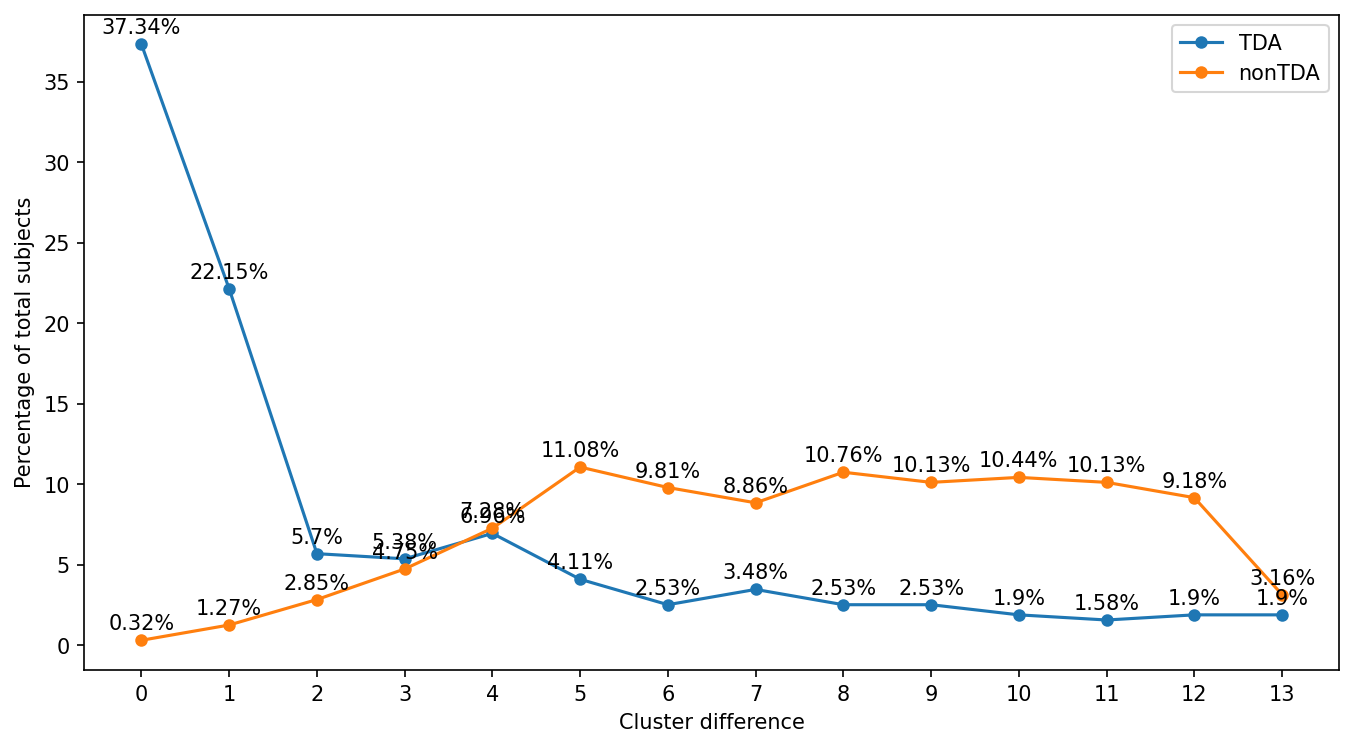
\includegraphics[width=0.8\textwidth]{figures/tda_nontda.png}\hfill
	\end{subfigure}
	\caption{Cluster distance comparison between TDA and nonTDA pipeline}
	\label{fig:clus_distance}
\end{figure}

We capture the number of clusters for 316 subjects for all three data cohorts for both pipelines. We calculate the distance between the number of clusters for each subject using: 

\begin{align}
    distance(subject_i) &= abs(subject_{i_{2500ms}} - subject_{i_{1400ms}})   \nonumber\\
    &+ abs(subject_{i_{1400ms}} - subject_{i_{645ms}})   \nonumber \\ 
    &+ abs(subject_{i_{645ms}} - subject_{i_{2500ms}}) \label{eq:dis}
\end{align}

where $subject_{i_{2500ms}}, subject_{i_{1400ms}}, subject_{i_{645ms}}$ are the number of clusters for $subject_i$ for the data cohorts $2500ms$, $1400ms$, $645ms$ respectively and $abs$ denotes the absolute difference. 
% Table \ref{tab:clustering} 
Figure \ref{fig:clus_distance} shows the distance analysis for both of the pipelines. In the TDA pipeline, we see that majority of the subjects ($59\%$) have a distance less than or equal to one for the data cohorts. On the other hand, in the nonTDA pipeline, less than $2\%$ of the subjects have a distance less than or equal to one. Thus, it shows the resiliency of the persistent homology-based techniques on rs-fMRI data analysis on different data acquisition parameters.




Additionally, we perform a pairwise comparison of the number of clusters for the data cohorts for both of the pipelines. The value of $abs(subject_{i_{2500ms}} - subject_{i_{1400ms}})$ represents the pairwise distance on the number of clusters for $subject_i$ for the data cohorts $2500ms$ and $1400ms$. Similarly, the value of $abs(subject_{i_{1400ms}} - subject_{i_{645ms}})$ and $abs(subject_{i_{645ms}} - subject_{i_{2500ms}})$ represent the pairwise distance on the number of clusters between the data cohorts ($1400ms$, $645ms$) and ($645ms$, $2500ms$) respectively. This pairwise comparison will help to identify whether there is a closer similarity between the data cohorts in the TDA pipeline over the nonTDA pipeline. Figure \ref{fig:clus_distance_pairwise} shows the pairwise distance between the data cohorts in the TDA pipeline. In this pipeline, the pairwise distance between data cohorts $1400ms$ and $645ms$ show the highest similarity ($78\%$ matching within distance 2). The data cohort pair $645ms$ and $2500ms$ has a similarity of $77\%$ within distance two, and data cohort pair $2500ms$ and $1400ms$ has a similarity of $74\%$ within the same distance. This high similarity between the data cohort pairs proves the efficacy of persistent homology-based techniques on the rs-fMRI data analysis with different temporal sampling periods. Table \ref{tab:nontda_between} shows the pairwise distance between the data cohorts in the traditional FCN analysis pipeline (nonTDA). Here, we see the maximum similarity between the data cohorts $1400ms$ and $645ms$ with $40\%$ similarity within distance 2. The other data cohort pairs (($2500ms$, $1400ms$) and ($645ms$, $2500ms$)) has $23\%$ and $22\%$ similarity within the same distance. This low similarity between the data cohorts using traditional FCN analysis indicates the inefficiency of the nonTDA pipeline for analysing rs-fMRI data with different data acquisition parameters. 


Overall, these results demonstrate that TDA captures fundamental temporal properties of rs-fMRI data that are robust to changes in sampling rate. By extracting topological features using persistent homology, TDA provides a more invariant representation of functional brain dynamics compared to traditional functional connectivity methods. This suggests TDA is a promising approach for analyzing complex temporal patterns in resting-state fMRI.




\setlength{\tabcolsep}{0.5em} % for the horizontal padding
{\renewcommand{\arraystretch}{1.2}% for the vertical padding
    \begin{table}[!ht]
        \centering
        \begin{tabular}
        {| c | c | c | c | c | c | c |}
         \hline
            \multirow{2}{*}{Distance} & \multicolumn{2}{c |}{$2500ms$ and $1400ms$ } & \multicolumn{2}{c |}{$1400ms$ and $645ms$ } & \multicolumn{2}{c |}{$645ms$ and $2500ms$ } \\ \cline{2-7}
              & Subjects & Percentage & Subjects & Percentage & Subjects & Percentage
             \\ \hline \hline
0 & 10 & 3.165\% & 39 & 12.342\% & 13 & 4.114\% \\ \hline 
1 & 31 & 9.810\% & 47 & 14.873\% & 23 & 7.278\% \\ \hline 
2 & 34 & 10.759\% & 41 & 12.975\% & 34 & 10.759\% \\ \hline 
3 & 31 & 9.810\% & 26 & 8.228\% & 32 & 10.127\% \\ \hline 
4 & 38 & 12.025\% & 35 & 11.076\% & 27 & 8.544\% \\ \hline 
5 & 37 & 11.709\% & 31 & 9.810\% & 18 & 5.696\% \\ \hline 
6 & 32 & 10.127\% & 24 & 7.595\% & 29 & 9.177\% \\ \hline 
7 & 18 & 5.696\% & 17 & 5.380\% & 22 & 6.962\% \\ \hline 
8 & 24 & 7.595\% & 25 & 7.911\% & 22 & 6.962\% \\ \hline 
9 & 16 & 5.063\% & 12 & 3.797\% & 20 & 6.329\% \\ \hline 
10 & 16 & 5.063\% & 7 & 2.215\% & 27 & 8.544\% \\ \hline 
11 & 18 & 5.696\% & 5 & 1.582\% & 22 & 6.962\% \\ \hline 
12 & 9 & 2.848\% & 4 & 1.266\% & 20 & 6.329\% \\ \hline 
13 & 2 & 0.633\% & 3 & 0.949\% & 7 & 2.215\% \\ \hline
        \end{tabular}
        \caption{Clustering result similarity between cohorts for non TDA pipeline}
        \label{tab:nontda_between}
    \end{table}      




\section{\textcolor{red}{Discussion}}
\label{sec:discussion}

MRI scanners across the world have different configurations and field strengths~\footnote{For example, the MRI machines available for research in the state of Alabama in the United States - Siemens 7T Magnetom and 3T Verio at Auburn University, Siemens 3T Prisma at the University of Alabama  Birmingham, Philips 3T Achieva at the University of South Alabama and Siemens 3T Prisma at the University of Alabama Tuscaloosa - all have different configurations}. Data acquired from different scanners with different parameters have some degree of noise in them due to non-neural variability introduced by different scanner configurations and data acquisition parameters, which makes it difficult for datasets acquired from different machines to be pooled into one large dataset for analysis within a single framework. As a result, conducting research on brain networks obtained from fMRI is primarily concentrated at localized sites. Such studies are limited by the fact that the number of subjects that can be scanned at a single scanner is limited, which tends to reduce the sample size and hence the generalizability of the results. This can be overcome by conducting multi-site studies with sites that are geographically closer to the population of interest. However, as mentioned above, data acquired from different scanners and parameters introduces noise, which reduces the effect of interest that is neural in origin, and hence reduces the utility of such a multi-site effort. Our paper aims to address precisely this aspect. Accordingly, we have proposed persistent homology-based techniques (which are based on TDA) as a means to overcome noise introduced by non-neural factors such as different data acquisition parameters and extract the inherent structural topology underlying brain networks characterized by fMRI. Computational topology is known to extract underlying shapes from complex data structures. We have shown that the topology-based metric for the brain network is invariant to data acquisition parameters such as sampling period. The metric captures the underlying shape of the brain network in topological space, thus creating a common ground to facilitate multi-site data-driven analysis of fMRI datasets (acquired from different scanners).

We were able to establish the efficacy of the TDA-based pipeline by comparing it against the traditional data analysis pipeline presented in Section III.D.3. In a traditional pipeline, raw FCNs are used directly instead of using a topological feature. The results of this pipeline are a strong indication that these traditional techniques are not able to establish similarity across FCNs of the same subjects acquired with different TRs and acquisition parameters. While the opposite was true for the TDA-based metric, wherein we showed both qualitatively and quantitatively that the metric remains statistically invariant across same subjects irrespective of the sampling period with which resting state fMRI data was acquired.
This demonstrates the utility of TDA-based analysis because, in principle, data acquired using different parameters from the same subject should still capture the same brain network. Certain limitations of our work must be kept in mind while interpreting the results. Even though the sampling period was different across the three different acquisitions, some other parameters such as number of volumes, multiband factor, FOV and voxel size also varied across the three cohorts. Ideally, we would want to investigate the limits of parameter variability that would show invariance in the TDA metric by varying only one parameter at a time. This will be part of our future work in this area. Also, future work can investigate whether the TDA metric is invariant to differences in other variables such as vendors (such as Siemens, GE and Philips) and scanner models within a given vendor.




\section{Conclusion}
\label{sec:conclusion}

In this study, we have demonstrated the effectiveness of Topological Data Analysis (TDA) in uncovering temporal properties within resting-state functional magnetic resonance imaging (rs-fMRI) data. Our research highlights TDA's robustness in the presence of varying temporal sampling rates, surpassing traditional connectivity analysis methods. Key findings emphasize TDA's remarkable stability, with 59\% of subjects consistently showing clustering results across different temporal sampling periods (2500ms, 1400ms, 645ms), compared to less than 2\% using traditional methods. TDA also reveals strong pairwise similarities between sampling periods, showcasing its ability to capture temporal dynamics. In conclusion, our study establishes TDA as a valuable tool for revealing temporal nuances in rs-fMRI data, offering a level of robustness unmatched by traditional methods. Through persistent homology, TDA provides a stable, invariant representation of dynamic brain connectivity, promising valuable insights into complex temporal patterns in resting-state fMRI data across diverse acquisition parameters. To promote reproducibility, we have made all our code, scripts, data, and documentation available at \url{https://github.com/harp-lab/TemporalBrainPH}.


\section{\textcolor{red}{Acknowledgment}}
We thank Xi-Nian Zuo from Beijing Normal University for sharing some of the data with us. We are also grateful to the entire Enhanced Nathan Kline Institute - Rockland Sample (NKI-RS) team for providing free access to the raw MRI data. Principal support for the enhanced NKI-RS project is provided by the NIMH BRAINS R01MH094639-01 (PI Milham). Funding for key personnel also provided in part by the New York State Office of Mental Health and Research Foundation for Mental Hygiene. Funding for the decompression and augmentation of administrative and phenotypic protocols provided by a grant from the Child Mind Institute (1FDN2012-1). Additional personnel support provided by the Center for the Developing Brain at the Child Mind Institute, as well as NIMH R01MH081218, R01MH083246, and R21MH084126. Project support also provided by the NKI Center for Advanced Brain Imaging (CABI), the Brain Research Foundation, and the Stavros Niarchos Foundation.


\bibliographystyle{IEEEtran}
\bibliography{PH}

\clearpage
\appendix
\section{Supplementary}

We extend our experiments by using the existing mapping for Pearson’s correlation coefficients $pcc(p, q)$. We use popular Pearson’s correlation coefficients $pcc(p, q)$ to measure the interrelation between any two data points (nodes) $p$ and $q$ in the fMRI data as it is independent on FCN construction method ~\cite{smith2011network}. This technique ensures that to map of the higher correlations between the data points to a smaller value. The mapping we used in extended experiments is:

\[
\mathit{d(p, q)} = 
1 - pcc(p, q)
\]

This mapping is used by the existing literature \cite{smith2011network, 7164127,lee2011discriminative, 6307875, edelsbrunner2008persistent}. This mapping ensures the distance dissimilarity for correlated and anti-correlated nodes. We run the TDA and nonTDA pipelines using this mapping and generates the clustering using both Wasserstein and Bottleneck distance.

\begin{figure}[!th]
	\centering
	\begin{subfigure}[!th]{1\textwidth}
		\centering
		\hspace{8mm}
		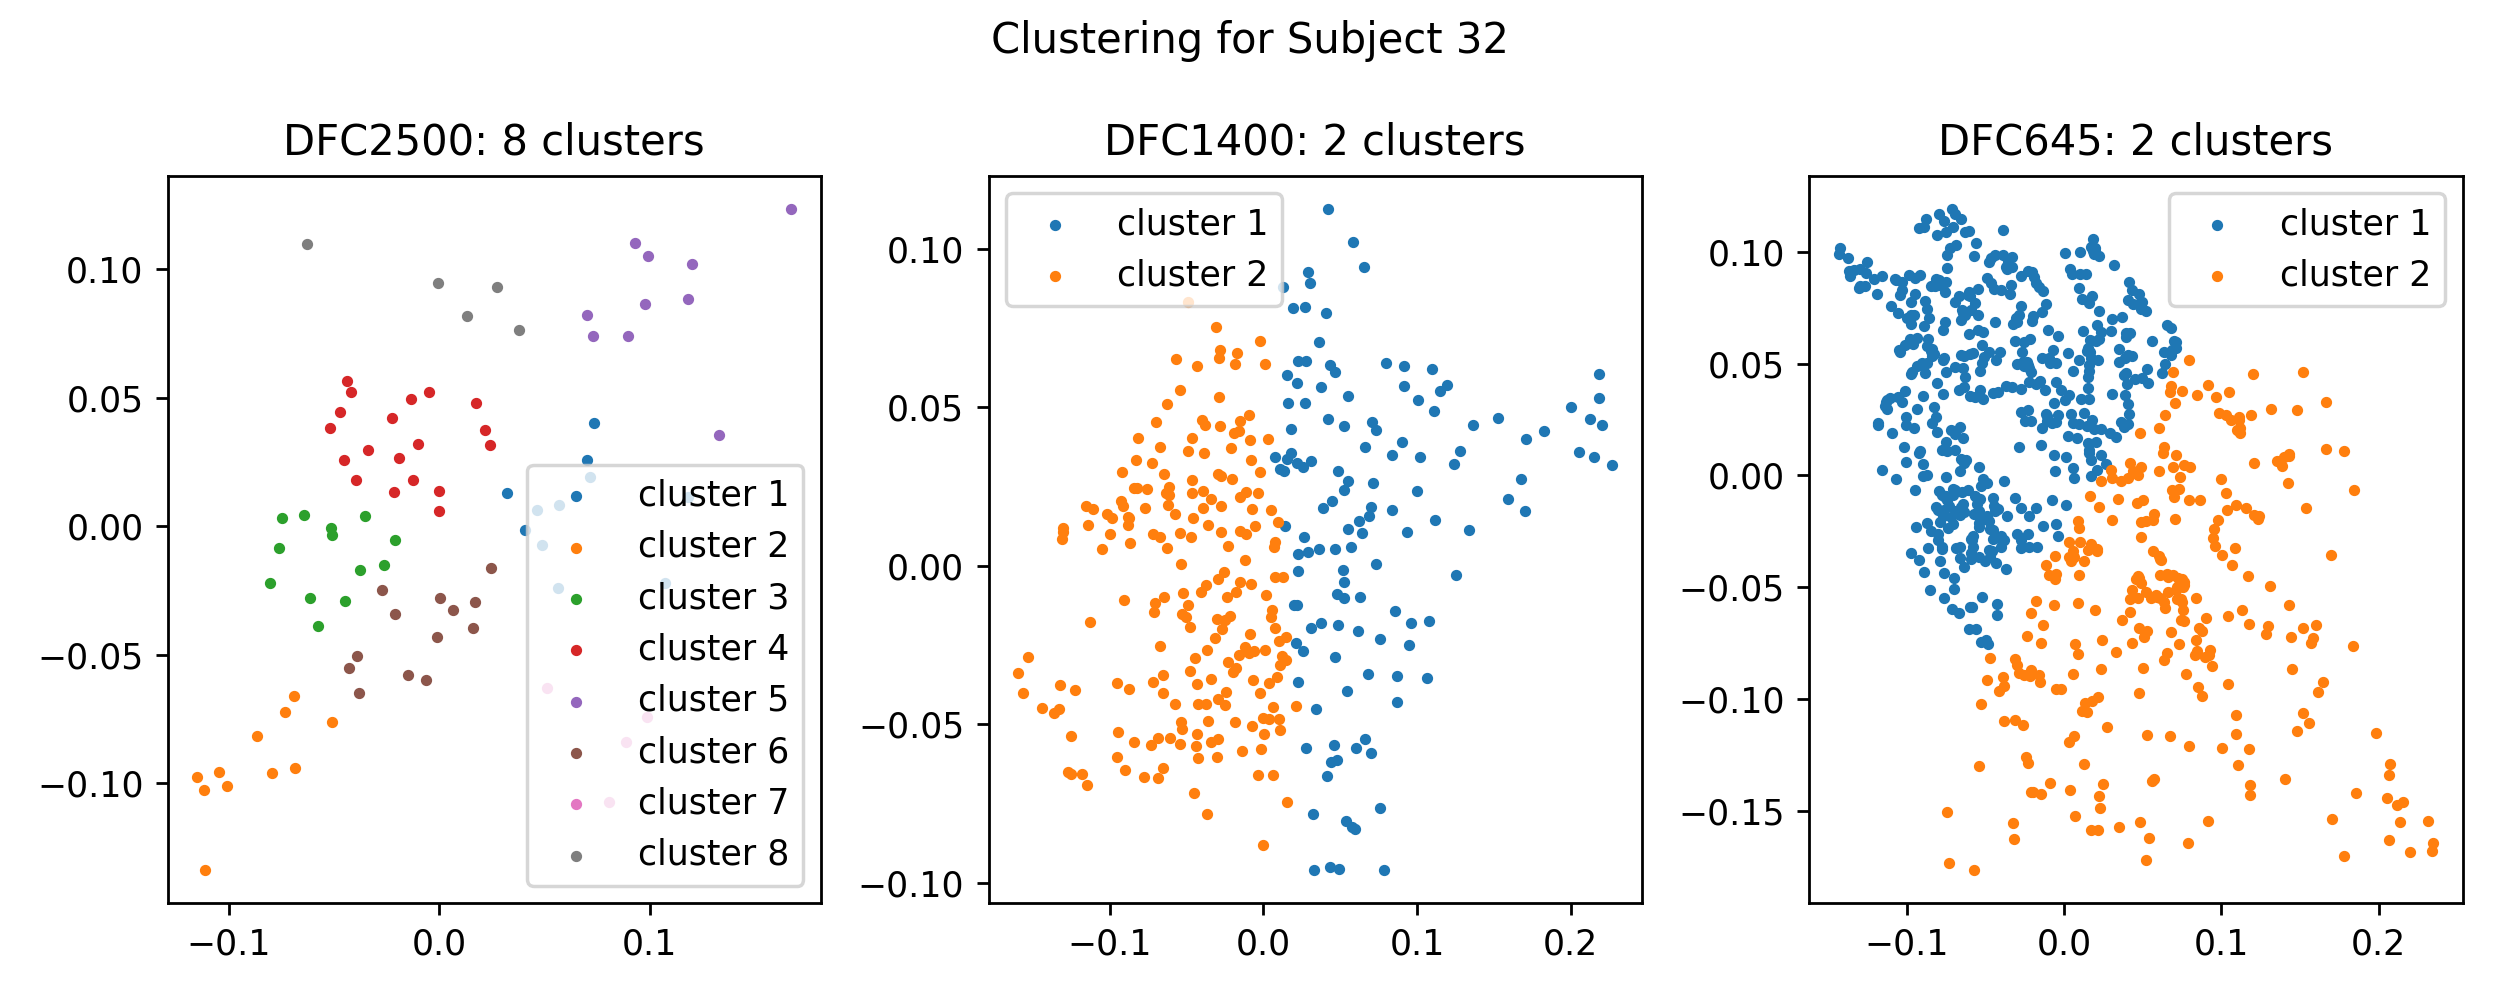
\includegraphics[width=1\textwidth, trim={0cm, 0.0cm, 0.0cm, 0.0cm}]{figures/new_formula_tda_bn_subject_32.png}\hfill
		%\hspace{-15mm}
	\end{subfigure}
	\begin{subfigure}[!th]{1\textwidth}
		\centering
		\hspace{8mm}
		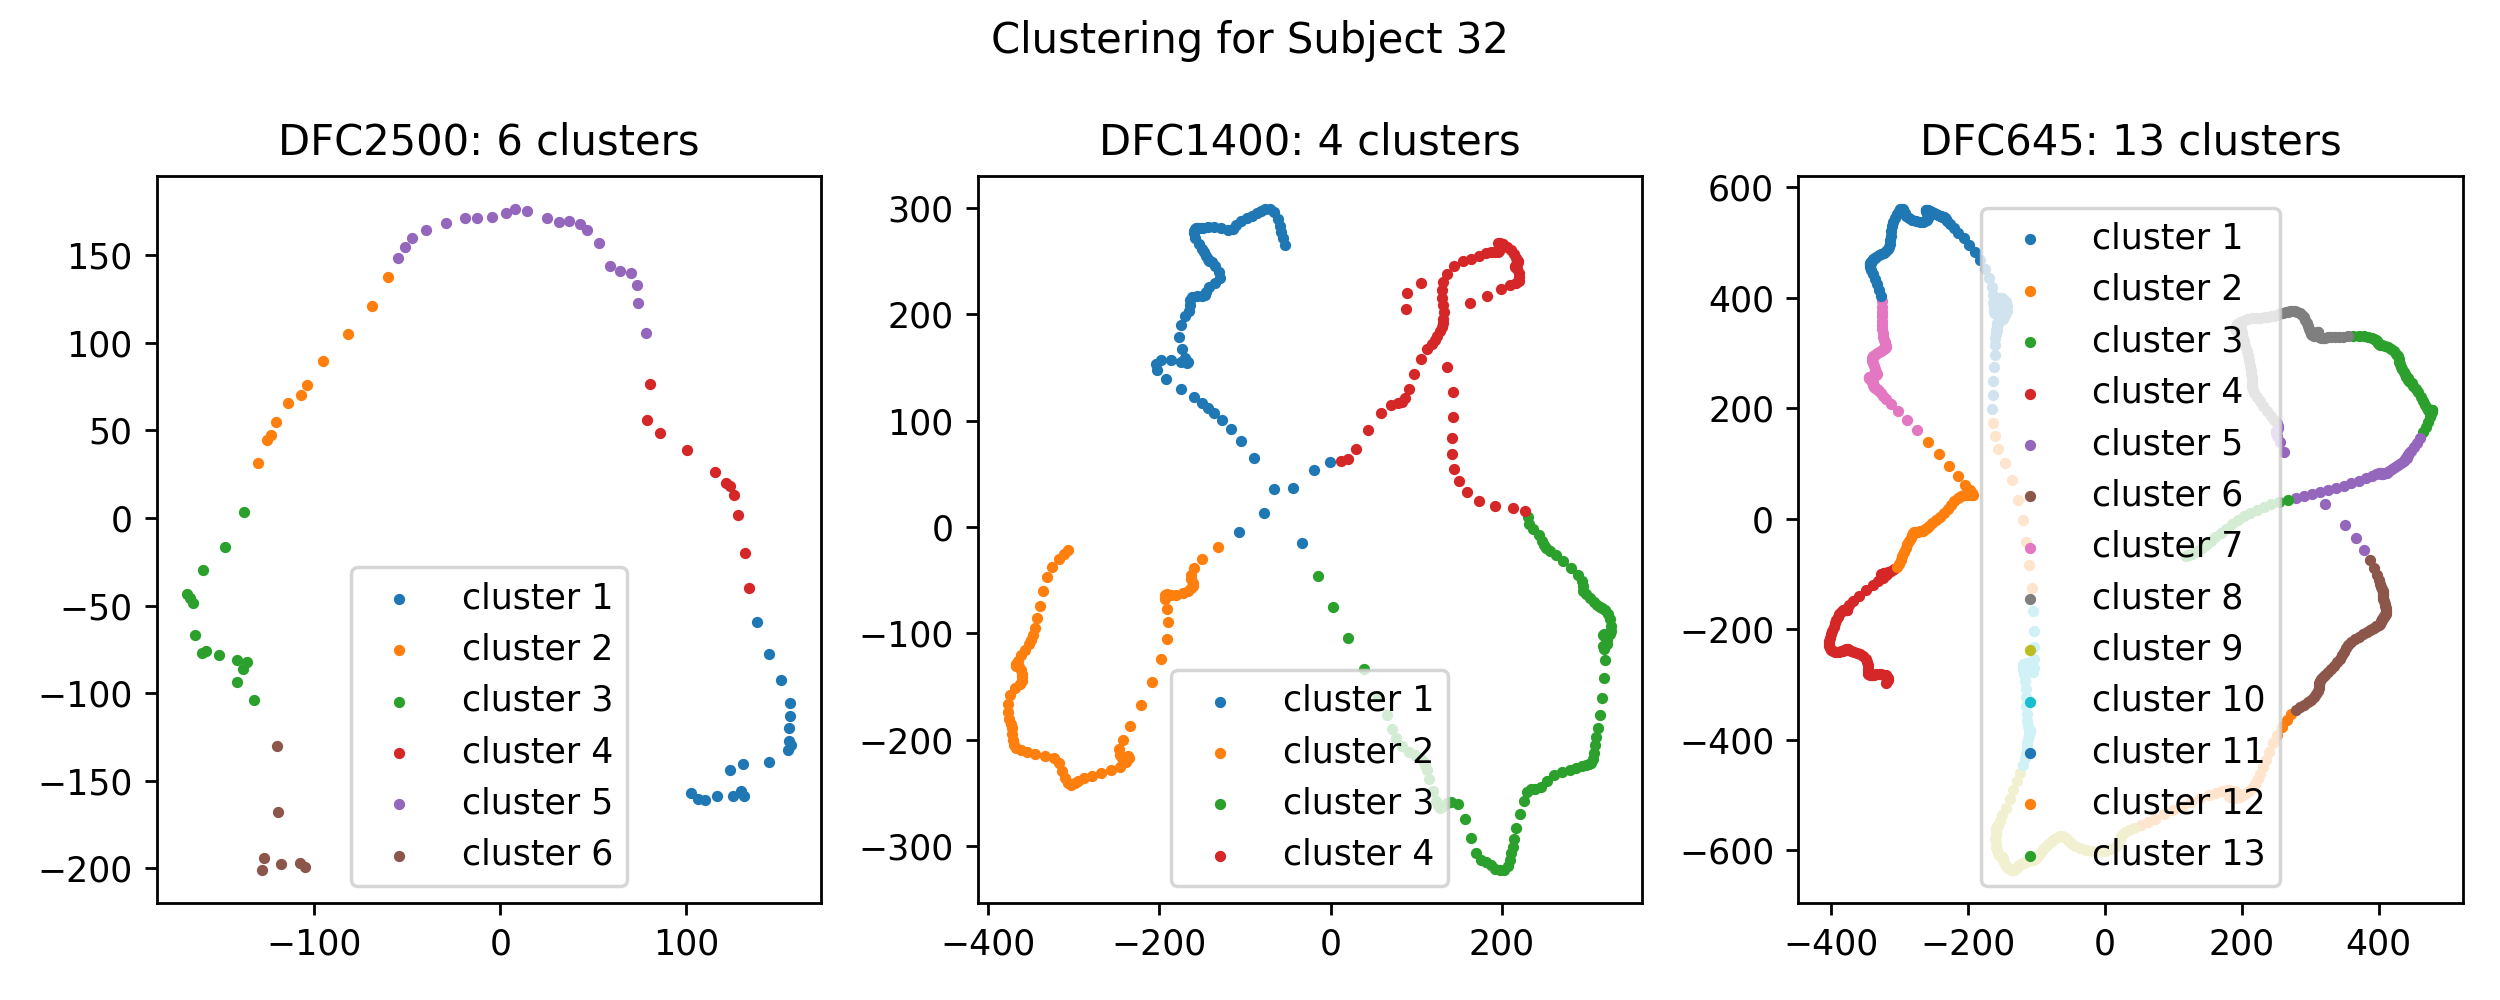
\includegraphics[width=1\textwidth, trim={0cm, 0.0cm, 0.0cm, 0.0cm}]{figures/new_formula_nontda_subject_32.png}\hfill
		%\hspace{-15mm}
	\end{subfigure}
	\caption{Clustering result for subject $32$ (top row) for temporal period $2500ms$ (left), $1400ms$ (center), and $645ms$ (right) using $1 - corr$ formula and Bottleneck distance. Clustering result for the same subject (bottom row) with NonTDA Clustering result.}
	\label{fig:clus_new_formula}
\end{figure}

Figure \ref{fig:clus_new_formula} shows the clustering result for a single subject (subject 32) for all three data cohorts ($2500ms$, $1400ms$, $645ms$). The top row of the figure represents the plotted clusters using the TDA pipeline using Bottleneck distance. The bottom row of the figure shows the plotted clusters for the same subject using the nonTDA pipeline, and the number of clusters varies for the data cohorts. 

\setlength{\tabcolsep}{0.5em} % for the horizontal padding
{\renewcommand{\arraystretch}{1.2}% for the vertical padding
    \begin{table}[!th]
        \centering
        \begin{tabular}
        {| c | c | c | c | c |}
         \hline
            \multirow{2}{*}{Distance} & \multicolumn{2}{c |}{TDA Pipeline} & \multicolumn{2}{c |}{NonTDA Pipeline} \\ \cline{2-5}
              & Subjects & Percentage & Subjects & Percentage
             \\ \hline \hline
             0 & 109 & 34.49\% & 4 & 1.27\% \\ \hline 
             1 & 50 & 15.82\% & 5 & 1.58\% \\ \hline 
             2 & 39 & 12.34\% & 11 & 3.48\% \\ \hline 
             3 & 26 & 8.23\% & 18 & 5.70\% \\ \hline 
             4 & 27 & 8.54\% & 22 & 6.96\% \\ \hline 
             5 & 11 & 3.48\% & 30 & 9.49\% \\ \hline 
             6 & 11 & 3.48\% & 20 & 6.33\% \\ \hline 
             7 & 5 & 1.58\% & 23 & 7.28\% \\ \hline 
             8 & 6 & 1.90\% & 39 & 12.34\% \\ \hline 
             9 & 5 & 1.58\% & 34 & 10.76\% \\ \hline 
             10 & 5 & 1.58\% & 36 & 11.39\% \\ \hline 
             11 & 6 & 1.90\% & 43 & 13.61\% \\ \hline 
             12 & 8 & 2.53\% & 21 & 6.65\% \\ \hline 
             13 & 8 & 2.53\% & 10 & 3.16\% \\ \hline 
             
        \end{tabular}
        \caption{Distance between the number of clusters for the data cohorts for TDA (BN) and NonTDA pipeline using Eq. \ref{eq:dis}}
         \label{tab:clustering_new_formula}
    \end{table}   

We capture the number of clusters for 316 subjects for all three data cohorts for both pipelines with this mapping using Equaltion \ref{eq:dis}. Table \ref{tab:clustering_new_formula} shows the distance analysis for both of the pipelines. In the TDA pipeline with Bottleneck distance, we see that majority of the subjects ($59\%$) have a distance less than or equal to one for the data cohorts. On the other hand, in the nonTDA pipeline, less than $3\%$ of the subjects have a distance less than or equal to one. We also perform a pairwise comparison of the number of clusters for the data cohorts for both of the pipelines. Table \ref{tab:tda_between_new_ws} shows the pairwise distance between the data cohorts in the TDA pipeline using Wasserstein distance. Table \ref{tab:tda_between_new_bn} shows the pairwise distance between the data cohorts in the TDA pipeline using Bottleneck distance. Table \ref{tab:nontda_between_new_eu} shows the pairwise distance between the data cohorts in the traditional FCN analysis pipeline (nonTDA). 

    \begin{table}[!th]
        \centering
        \begin{tabular}
        {| c | c | c | c | c | c | c |}
         \hline
            \multirow{2}{*}{Distance} & \multicolumn{2}{c |}{$2500ms$ and $1400ms$ } & \multicolumn{2}{c |}{$1400ms$ and $645ms$ } & \multicolumn{2}{c |}{$645ms$ and $2500ms$ } \\ \cline{2-7}
              & Subjects & Percentage & Subjects & Percentage & Subjects & Percentage
             \\ \hline \hline
0 & 120 & 37.975\% & 100 & 31.646\% & 123 & 38.924\% \\ \hline 
1 & 51 & 16.139\% & 49 & 15.506\% & 44 & 13.924\% \\ \hline 
2 & 24 & 7.595\% & 32 & 10.127\% & 19 & 6.013\% \\ \hline 
3 & 19 & 6.013\% & 18 & 5.696\% & 21 & 6.646\% \\ \hline 
4 & 15 & 4.747\% & 15 & 4.747\% & 15 & 4.747\% \\ \hline 
5 & 14 & 4.430\% & 12 & 3.797\% & 15 & 4.747\% \\ \hline 
6 & 13 & 4.114\% & 10 & 3.165\% & 13 & 4.114\% \\ \hline 
7 & 13 & 4.114\% & 19 & 6.013\% & 12 & 3.797\% \\ \hline 
8 & 4 & 1.266\% & 8 & 2.532\% & 5 & 1.582\% \\ \hline 
9 & 7 & 2.215\% & 9 & 2.848\% & 10 & 3.165\% \\ \hline 
10 & 10 & 3.165\% & 10 & 3.165\% & 14 & 4.430\% \\ \hline 
11 & 11 & 3.481\% & 7 & 2.215\% & 4 & 1.266\% \\ \hline 
12 & 6 & 1.899\% & 8 & 2.532\% & 8 & 2.532\% \\ \hline 
13 & 9 & 2.848\% & 19 & 6.013\% & 13 & 4.114\% \\ \hline 
        \end{tabular}
        \caption{Clustering result similarity between cohorts for TDA pipeline using 1 - correlation formula and WS distance}
        \label{tab:tda_between_new_ws}
    \end{table}    
    

    \begin{table}[!th]
        \centering
        \begin{tabular}
        {| c | c | c | c | c | c | c |}
         \hline
            \multirow{2}{*}{Distance} & \multicolumn{2}{c |}{$2500ms$ and $1400ms$ } & \multicolumn{2}{c |}{$1400ms$ and $645ms$ } & \multicolumn{2}{c |}{$645ms$ and $2500ms$ } \\ \cline{2-7}
              & Subjects & Percentage & Subjects & Percentage & Subjects & Percentage
             \\ \hline \hline
0 & 143 & 45.253\% & 189 & 59.810\% & 141 & 44.620\% \\ \hline 
1 & 52 & 16.456\% & 41 & 12.975\% & 45 & 14.241\% \\ \hline 
2 & 44 & 13.924\% & 28 & 8.861\% & 37 & 11.709\% \\ \hline 
3 & 19 & 6.013\% & 16 & 5.063\% & 21 & 6.646\% \\ \hline 
4 & 21 & 6.646\% & 8 & 2.532\% & 23 & 7.278\% \\ \hline 
5 & 5 & 1.582\% & 8 & 2.532\% & 10 & 3.165\% \\ \hline 
6 & 5 & 1.582\% & 7 & 2.215\% & 6 & 1.899\% \\ \hline 
7 & 4 & 1.266\% & 1 & 0.316\% & 4 & 1.266\% \\ \hline 
8 & 6 & 1.899\% & 3 & 0.949\% & 4 & 1.266\% \\ \hline 
9 & 3 & 0.949\% & 6 & 1.899\% & 7 & 2.215\% \\ \hline 
10 & 1 & 0.316\% & 2 & 0.633\% & 4 & 1.266\% \\ \hline 
11 & 5 & 1.582\% & 5 & 1.582\% & 5 & 1.582\% \\ \hline 
12 & 3 & 0.949\% & 2 & 0.633\% & 4 & 1.266\% \\ \hline 
13 & 5 & 1.582\% & 0 & 0.000\% & 5 & 1.582\% \\ \hline 
        \end{tabular}
        \caption{Clustering result similarity between cohorts for TDA pipeline using 1 - correlation formula and BN distance}
        \label{tab:tda_between_new_bn}
    \end{table}    


    \begin{table}[!th]
        \centering
        \begin{tabular}
        {| c | c | c | c | c | c | c |}
         \hline
            \multirow{2}{*}{Distance} & \multicolumn{2}{c |}{$2500ms$ and $1400ms$ } & \multicolumn{2}{c |}{$1400ms$ and $645ms$ } & \multicolumn{2}{c |}{$645ms$ and $2500ms$ } \\ \cline{2-7}
              & Subjects & Percentage & Subjects & Percentage & Subjects & Percentage
             \\ \hline \hline
0 & 21 & 6.646\% & 37 & 11.709\% & 12 & 3.797\% \\ \hline 
1 & 29 & 9.177\% & 36 & 11.392\% & 21 & 6.646\% \\ \hline 
2 & 43 & 13.608\% & 40 & 12.658\% & 27 & 8.544\% \\ \hline 
3 & 28 & 8.861\% & 39 & 12.342\% & 29 & 9.177\% \\ \hline 
4 & 38 & 12.025\% & 39 & 12.342\% & 34 & 10.759\% \\ \hline 
5 & 30 & 9.494\% & 29 & 9.177\% & 30 & 9.494\% \\ \hline 
6 & 23 & 7.278\% & 22 & 6.962\% & 14 & 4.430\% \\ \hline 
7 & 18 & 5.696\% & 20 & 6.329\% & 22 & 6.962\% \\ \hline 
8 & 20 & 6.329\% & 22 & 6.962\% & 26 & 8.228\% \\ \hline 
9 & 18 & 5.696\% & 17 & 5.380\% & 25 & 7.911\% \\ \hline 
10 & 16 & 5.063\% & 9 & 2.848\% & 23 & 7.278\% \\ \hline 
11 & 22 & 6.962\% & 3 & 0.949\% & 33 & 10.443\% \\ \hline 
12 & 6 & 1.899\% & 1 & 0.316\% & 15 & 4.747\% \\ \hline 
13 & 4 & 1.266\% & 2 & 0.633\% & 5 & 1.582\% \\ \hline 
        \end{tabular}
        \caption{Clustering result similarity between cohorts for NON TDA pipeline using 1 - correlation formula and EU distance}
        \label{tab:nontda_between_new_eu}
    \end{table}        
      



\end{document}
